%% 
%% Copyright 2007-2024 Elsevier Ltd
%% 
%% This file is part of the 'Elsarticle Bundle'.
%% ---------------------------------------------
%% 
%% It may be distributed under the conditions of the LaTeX Project Public
%% License, either version 1.3 of this license or (at your option) any
%% later version.  The latest version of this license is in
%%    http://www.latex-project.org/lppl.txt
%% and version 1.3 or later is part of all distributions of LaTeX
%% version 1999/12/01 or later.
%% 
%% The list of all files belonging to the 'Elsarticle Bundle' is
%% given in the file `manifest.txt'.
%% 
%% Template article for Elsevier's document class `elsarticle'
%% with numbered style bibliographic references
%% SP 2008/03/01
%% $Id: elsarticle-template-num.tex 249 2024-04-06 10:51:24Z rishi $
%%
% \documentclass[preprint,12pt,draft]{elsarticle}

%% Use the option review to obtain double line spacing
%% \documentclass[authoryear,preprint,review,12pt]{elsarticle}

%% Use the options 1p,twocolumn; 3p; 3p,twocolumn; 5p; or 5p,twocolumn
%% for a journal layout:
% \documentclass[draft,1p,times]{elsarticle}
% \documentclass[final,1p,times,sort&compress]{elsarticle}
% \documentclass[final,1p,times,twocolumn]{elsarticle}
\documentclass[final,3p,times,sort&compress]{elsarticle}
%% \documentclass[final,3p,times,twocolumn]{elsarticle}
% \documentclass[final,5p,times]{elsarticle}
% \documentclass[final,5p,times,twocolumn]{elsarticle}

%% For including figures, graphicx.sty has been loaded in
%% elsarticle.cls. If you prefer to use the old commands
%% please give \usepackage{epsfig}
%% 主要数学宏包
\usepackage{amsmath}     % 数学公式环境
\usepackage{amssymb}     % 提供 \mathbb 等数学符号
\usepackage{stmaryrd}    % 提供额外的数学符号
\usepackage{mathrsfs}    % 提供花体字母
\usepackage{tabularx}    % 可调列宽的表格
\usepackage{array}       % 提供高级列格式功能}
%% 图形、表格相关宏包
\usepackage{graphicx}    % 插入图像
\usepackage{caption}     % 修改图表标题
\usepackage{subcaption}  % 子图功能
\usepackage{multirow}    % 表格中单元格合并功能
\usepackage{booktabs}    % 提供 \toprule, \midrule, \bottomrule
\usepackage{tabularx}    % 可调列宽的表格
\usepackage{array}       % 提供高级列格式功能
\usepackage{float}       % 提供 [H] 位置选项
\usepackage{XeCJK}       % 提供中文支持
%% 参考文献、链接相关宏包
\usepackage{hyperref}    % 创建可点击的交叉引用和链接
\hypersetup{             % 超链接设置
    colorlinks=true,
    linkcolor=blue,
    citecolor=blue,
    filecolor=magenta,      
    urlcolor=blue,
}

% 注意：cleveref 宏包必须放在 hyperref 宏包的【后面】加载！
\usepackage[capitalize,nameinlink]{cleveref}

%% 排版和图文混排
\usepackage{wrapfig}     % 实现图文并排，将图片排版在文字右边

%% 颜色和样式
\usepackage{xcolor}      % 提供颜色支持

%% 算法相关宏包
\usepackage{algorithm}   % 算法环境
\usepackage{algorithmic} % 算法的伪代码支持

%% 可选宏包（根据需求决定是否使用）
% \usepackage{amsthm}     % 提供定理环境

%% The lineno packages adds line numbers. Start line numbering with
%% \begin{linenumbers}, end it with \end{linenumbers}. Or switch it on
%% for the whole article with \linenumbers.
\usepackage{lineno}

\journal{Nuclear Engineering and Technology}
% \journal{J. Comput. Phys.}
% \journal{Nat. Comput. Sci.}
% \journal{Comput. Methods Appl. Mech. Eng.}

\begin{document}
% \linenumbers
\begin{frontmatter}

    %% Title, authors and addresses

    %% use the tnoteref command within \title for footnotes;
    %% use the tnotetext command for theassociated footnote;
    %% use the fnref command within \author or \affiliation for footnotes;
    %% use the fntext command for theassociated footnote;
    %% use the corref command within \author for corresponding author footnotes;
    %% use the cortext command for theassociated footnote;
    %% use the ead command for the email address,
    %% and the form \ead[url] for the home page:
    %% \title{Title\tnoteref{label1}}
    %% \tnotetext[label1]{}
    %% \author{Name\corref{cor1}\fnref{label2}}
    %% \ead{email address}
    %% \ead[url]{home page}
    %% \fntext[label2]{}
    %% \cortext[cor1]{}
    %% \affiliation{organization={},
    %%             addressline={},
    %%             city={},
    %%             postcode={},
    %%             state={},
    %%             country={}}
    %% \fntext[label3]{}

   \title{面向非均匀介质中子扩散计算的变域积分弱解深度学习方法}

    \author[1]{Yang Liu}
    \ead{mathliuyang@163.com}

    \author[1,2]{Dong Liu\corref{cor1}}
    \ead{liudong@npic.ac.cn}

    \author[1]{Junfeng Wang}
    \ead{wangjf@scu.edu.cn}

    \author[2]{Zhen Liao}
    \ead{npicliaozhen@163.com}

    \author[2]{Kangjun He}
    \ead{820982892@qq.com}

    \author[1]{Zhenyu Liu}
    \ead{zhenyuliuchn@foxmail.com}

    \author[2]{Chao Wu}
    \ead{22031110387@stu.xidian.edu.cn}

    \author[2]{Xiyan Zhai}
    \ead{zhai2454814@gmail.com}

    \cortext[cor1]{Corresponding author}

    \affiliation[1]{organization={College of Computer Science, Sichuan University},
        % addressline={},
        city={Chengdu 610065},
        % postcode={610065},
        % state={Sichuan},
        country={China}}

    \affiliation[2]{organization={State Key Laboratory of Advanced Nuclear Energy Technology, Nuclear Power Institute of China},
        % addressline={},
        city={Chengdu 610213},
        % postcode={610213},
        % state={Sichuan},
        country={China}}


    % \affiliation[3]{organization={School of Information and Software Engineering, University of Electronic Science and Technology of China},
    %       % addressline={},
    %       city={Chengdu 610031},
    %       % postcode={610031},
    %       % state={Sichuan},
    %       country={China}}

    % \affiliation[3]{organization={Science and Technology Committee, China National Nuclear Corporation},
    %       addressline={},
    %       city={Beijing},
    %       postcode={100045},
    %       state={},
    %       country={China}}

    %% Abstract

\begin{abstract}
中子扩散计算是反应堆物理分析、堆芯设计与安全评估中的关键环节。实际堆芯通常由多种材料组成，扩散系数与宏观截面往往具有不连续分布的特性。利用深度学习方法进行非均匀介质中子扩散计算时，界面处系数的不连续性会导致数值解产生奇异性，进而引发收敛困难等问题。
针对上述问题，本文将变域积分弱解（VIWS）理论引入非均匀介质中子扩散深度学习计算，给出了适合复杂几何、多群条件下的中子扩散方程变域积分弱解具体形式，降低了方程微分项的阶数，消除了界面系数不连续带来的奇异性；构建了适用于固定源与特征值问题的无网格深度学习计算框架，基于单一神经网络在全求解域上构建了深度学习损失函数，避免了在材料界面上的额外数值处理，从而降低了深度学习计算的复杂性。进一步采用原函数变换，将弱解形式方程中带有连续核的积分项变换为微分形式，提升了深度学习计算效率。多个典型算例的数值结果表明，所提方法能够有效求解二维与三维非均匀介质中子扩散问题，对复杂几何、多群、特征值求解等重要问题均具有良好的适应性。本文工作提供了中子扩散计算新的技术途径，为中子扩散方程深度学习方法的工程应用奠定了良好的技术基础。
\end{abstract}
    %%Graphical abstract
    % \begin{graphicalabstract}
    % \includegraphics[width=1\textwidth]{./Graphical abstract.png}
    % \end{graphicalabstract}


    %%Research highlights
    % \begin{highlights}
    % \item Research highlight 1
    % \item Research highlight 2
    % \end{highlights}

    %% Keywords
    \begin{keyword}
        中子扩散计算 \sep 深度学习 \sep 变域积分弱解 \sep 非均匀介质 \sep 原函数变换

        %% PACS codes here, in the form: \PACS code \sep code

        %% MSC codes here, in the form: \MSC code \sep code
        %% or \MSC[2008] code \sep code (2000 is the default)

    \end{keyword}

\end{frontmatter}

%% Add \usepackage{lineno} before \begin{document} and uncomment 
%% following line to enable line numbers
%% \linenumbers

%% main text
%%
\section{引言 (Introduction)} 
\label{sec:introduction}

中子通量分布与临界特征值的准确预测是反应堆堆芯设计、燃料管理和安全裕度评估中的基础问题。作为中子输运方程在工程尺度上的经典近似，中子扩散方程兼具物理可解释性和计算效率，长期用于反应堆物理分析\cite{stacey2018nuclear, XieZhongSheng2020HeFanYing}。实际堆芯通常由燃料、包壳、慢化剂、反射层和控制棒等多种材料组成，扩散系数与宏观截面在材料界面处呈分段突变。受界面条件约束，中子通量保持连续，而其法向梯度随扩散系数的变化而发生跳变。由此产生的界面奇异性，是复杂非均匀介质中子扩散计算中亟待重点处理的问题。

{\color{black}
针对中子扩散方程，传统数值方法已形成较为成熟的技术体系，主要包括有限差分法（FDM）\cite{zhu2016optimally, mohamedhamada2022higher}、有限体积法（FVM）\cite{li2024research}、有限元法（FEM）\cite{chunyu2018fast, zong2023multithreaded}以及各类节点法\cite{wang2010improved, yin2024efficient, zhuang2021variational}。这些方法在反应堆工程计算中具有较高可靠性，并已在现有堆型分析与设计中得到广泛应用。但随着未来反应堆堆芯几何结构更加复杂、布局更加紧凑，中子各向异性进一步增强，发展高维高精度，几何适应性强、兼具连续场表达能力和界面处理能力的无网格计算方法，仍是工业界持续关注的重点与难点。}

近年来，以物理信息神经网络（PINNs）\cite{raissi2019physicsinformed}为代表的基于深度学习的微分方程数值方法在复杂非线性偏微分方程求解中显示出一定优势，并已应用于多个学科问题\cite{karniadakis2021physicsinformed,cuomo2022scientific,toscano2025pinns,luo2025physicsinformed}。
特别地，在反应堆物理领域，PINN 已被用于多维中子扩散计算、反应堆动力学、瞬态分析和临界特征值问题\cite{elhareef2021physicsinformed,xie2021neural,LiuDong2022JiYupinnShen,schiassi2022physicsinformed,prantikos2023physicsinformed,liu2024deep,lee2026development,zeng2026application}。然而，现有的深度学习方法在处理不连续系数问题时仍面临明显困难：
一方面，系数的突变使得解的光滑性假设失效；另一方面，由于在逼近高频特征时存在固有的谱偏差，这些方法难以精确捕捉界面附近的梯度跃变\cite{haghighat2021physicsinformed,lu2021deepxde}。
{\color{black}
为了解决这些问题，已有研究提出了多种改进策略，大体可归纳为三类。第一类方法采用区域分解策略，使用多个神经网络分别表示不同子域内的解，并通过通量连续性等界面条件实现子域耦合\cite{jagtap2020conservative, d.jagtap2020extended,li2020deep,he2022meshfree,wu2022inn,mistani2023jaxdips}。第二类方法保持单一网络结构，通过调整界面附近采样点密度或引入残差重采样机制，提高网络对局部非光滑区域的分辨能力\cite{xie2022weighted,xie2021neural}。第三类方法同样基于单一网络框架，但通过设计特殊激活函数\cite{sarma2024interface,roy2025adaptive}或构造专门的界面损失函数\cite{yao2023deep,tseng2023cuspcapturing,li2025continuitypreserved,li2025two}来刻画界面跳变特征。总体而言，虽然第二类方法实现简单，但由于界面导数的奇异性问题，其往往难以捕捉不连续特征，导致精度大幅下降。而第一类和第三类方法在简单界面问题上具有更好的精度和效率，但在应用于多区域或复杂几何时，计算复杂度较高。每个界面都需要专门的处理，这必然导致性能下降。针对中子扩散问题，也有研究发展了守恒型 PINN（cPINN）、数据赋能 PINN（DEPINN）和残差重采样物理信息神经网络（$\mathrm{R}^2$-PINN）等方法\cite{wang2022surrogate,yang2023physicsconstrained,yang2023dataenabled,yang2024uncertainty,heng2026residual}。这些方法一定程度上改善了训练稳定性和求解精度，但在界面密集的复杂堆芯几何中，往往仍需依赖区域分解、多网络耦合或先验数据。因此，如何在单一全局网络框架下有效处理不连续系数引起的界面奇异性，仍是深度学习中子扩散计算中亟需解决的问题\cite{xie2024physicsspecialized,liu2024discontinuity}。}

{\color{black} 最近，文献 \cite{LiuDong2025MianXiangShen} 提出的变域积分弱解方法（Variable-domain Integral Weak Solution, VIWS）为不连续系数偏微分方程的深度学习求解提供了新的思路。该方法不同于传统的固定区域积分弱解形式，其核心在于以变域积分弱形式替代强形式残差，从而降低材料界面处梯度跳变对网络训练的影响。然而，已有 VIWS 研究仅给出了变域积分弱解的基本数理形式\cite{LiuDong2025MianXiangShen, LiuDong2026MianXiangShen}，缺乏对中子扩散方程的详细推导及完整形式，特别是对于高维多群、复杂几何、特征值搜索等反应堆工程中子扩散计算涉及的重要问题尚未进行充分验证。为此，本文将 VIWS 理论拓展至非均匀介质中子扩散计算，构建了适合复杂中子扩散计算的深度学习框架，并通过具有工程特点的中子扩散计算典型算例，验证与评价 VIWS 理论及其相关数值计算方法的性能和在反应堆工程上的适用性。}

本文其余部分安排如下：第二节给出中子扩散方程的数学模型，重点介绍多群固定源问题、特征值问题及非均匀介质界面条件；第三节构建中子扩散方程的变域积分弱形式，并给出原函数变换及相应的深度学习求解框架；第四节通过多个二维和三维数值算例验证所提方法在复杂几何、多群耦合和特征值计算中的性能；第五节总结全文并展望后续研究方向。

\section{中子扩散方程} 
\label{sec:neutron_diffusion_equation}

中子扩散方程是中子输运方程在工程尺度上的常用近似，也是反应堆物理分析和堆芯设计中的基础模型。它描述中子在介质中的扩散、吸收、散射和裂变产生过程。其连续能量形式可写为 \cite{XieZhongSheng2020HeFanYing}
\begin{equation}
    \begin{aligned}
        \frac{1}{v} \frac{\partial \phi(\boldsymbol{r}, E, t)}{\partial t}
        = & \ \nabla \cdot \left(D(\boldsymbol r,E)\nabla \phi(\boldsymbol{r}, E, t)\right)
        -\Sigma_{\mathrm{t}}(\boldsymbol{r}, E) \phi(\boldsymbol{r}, E, t)                            \\
          & +\int_0^{\infty} \Sigma_{\mathrm{s}}\left(\boldsymbol{r}, E^{\prime} \rightarrow E\right)
        \phi\left(\boldsymbol{r}, E^{\prime}, t\right) \mathrm{d} E^{\prime}                          \\
          & +\chi(E) \int_0^{\infty} \nu\left(E^{\prime}\right)
        \Sigma_{\mathrm{f}}\left(\boldsymbol{r}, E^{\prime}\right)
        \phi\left(\boldsymbol{r}, E^{\prime}, t\right) \mathrm{d} E^{\prime}
        +S(\boldsymbol{r}, E, t),
    \end{aligned}
    \label{eq:diffusion}
\end{equation}
其中，$\phi(\boldsymbol r,E,t)$ 为中子通量，$v$ 为中子速率，$D$ 为扩散系数，$\nu$ 为平均裂变中子数，$\chi(E)$ 为裂变中子能谱，$\Sigma_{\mathrm t}$、$\Sigma_{\mathrm s}$ 和 $\Sigma_{\mathrm f}$ 分别为总截面、散射截面和裂变截面，$S$ 为外源项。

实际计算中通常关心稳态问题。忽略时间项，并将连续能量变量离散为 $G$ 个能群，可得稳态多群固定源扩散方程：
\begin{equation}
    -\nabla\cdot \left( D_g(\boldsymbol r)\nabla\phi_g(\boldsymbol r) \right)
    + \Sigma_{\mathrm{t},g}(\boldsymbol r)\phi_g(\boldsymbol r)
    =
    \sum_{g'=1}^{G}
    \Sigma_{\mathrm{s},g'\to g}(\boldsymbol r)\phi_{g'}(\boldsymbol r)
    + \chi_g \sum_{g'=1}^{G}
    \left(\nu\Sigma_{\mathrm{f}}\right)_{g'}(\boldsymbol r)\phi_{g'}(\boldsymbol r)
    + S_g(\boldsymbol r),
    \qquad g=1,2,\ldots,G .
    \label{eq:multigroup_fixed_source}
\end{equation}
式中，$\phi_g$、$D_g$ 与 $S_g$ 分别为第 $g$ 群的中子通量、扩散系数和外源项；$\Sigma_{\mathrm{t},g}$、$\Sigma_{\mathrm{s},g'\to g}$、$\left(\nu\Sigma_{\mathrm{f}}\right)_{g'}$ 与 $\chi_g$ 分别代表总截面、由第 $g'$ 群散射至第 $g$ 群的散射截面、第 $g'$ 群的裂变产生截面和裂变谱份额。

当外源项为零时，堆芯临界特性可由有效增殖因子 $k_{\mathrm{eff}}$ 描述。此时，多群扩散方程可写为特征值问题：
\begin{equation}
    -\nabla\cdot \left( D_g(\boldsymbol r)\nabla\phi_g(\boldsymbol r) \right)
    + \Sigma_{\mathrm{t},g}(\boldsymbol r)\phi_g(\boldsymbol r)
    =
    \sum_{g'=1}^{G}
    \Sigma_{\mathrm{s},g'\to g}(\boldsymbol r)\phi_{g'}(\boldsymbol r)
    + \frac{\chi_g}{k_{\mathrm{eff}}}
    \sum_{g'=1}^{G}
    \left(\nu\Sigma_{\mathrm{f}}\right)_{g'}(\boldsymbol r)\phi_{g'}(\boldsymbol r),
    \qquad g=1,2,\ldots,G .
    \label{eq:multigroup_eigenvalue}
\end{equation}
其中，$k_{\mathrm{eff}}<1$、$k_{\mathrm{eff}}=1$ 和 $k_{\mathrm{eff}}>1$ 分别对应次临界、临界和超临界状态。

为保证问题适定，还需在边界 $\partial\Omega$ 上给定边界条件。常见边界条件可统一写为
\begin{equation}
    \alpha_g(\boldsymbol r)\phi_g(\boldsymbol r)
    + \beta_g(\boldsymbol r)D_g(\boldsymbol r)
    \nabla\phi_g(\boldsymbol r)\cdot\boldsymbol n
    = q_g(\boldsymbol r),
    \qquad \boldsymbol r\in\partial\Omega ,
    \label{eq:mg_bc}
\end{equation}
其中，$\boldsymbol n$ 为边界单位外法向量。通过选取不同的 $\alpha_g$、$\beta_g$ 和 $q_g$，可表示给定通量边界、给定法向流边界、反射边界和真空边界等情况。

实际堆芯由多种材料组成，扩散系数和宏观截面在不同材料区内取值不同。设计算域 $\Omega$ 被划分为 $M$ 个互不重叠的子区域：
\begin{equation}
    \Omega=\bigcup_{m=1}^{M}\Omega_m, \qquad
    \Omega_i^\circ\cap\Omega_j^\circ=\varnothing,\quad i\neq j.
    \label{eq:domain_decomposition}
\end{equation}
在子域 $\Omega_m$ 内，材料参数可表示为
\begin{equation}
    D_g(\boldsymbol r)=D_g^{(m)},\quad
    \Sigma_{\mathrm t,g}(\boldsymbol r)=\Sigma_{\mathrm t,g}^{(m)},\quad
    \Sigma_{\mathrm s,g'\rightarrow g}(\boldsymbol r)=\Sigma_{\mathrm s,g'\rightarrow g}^{(m)},\quad
    \Sigma_{\mathrm f,g}(\boldsymbol r)=\Sigma_{\mathrm f,g}^{(m)},
    \qquad \boldsymbol r\in\Omega_m.
    \label{eq:piecewise_coefficients}
\end{equation}
因此，在材料界面
\begin{equation}
    \Gamma_{ij}=\partial\Omega_i\cap\partial\Omega_j
\end{equation}
处，材料参数通常发生跳变。根据中子守恒，界面两侧应满足
\begin{equation}
    [\phi_g]_{\Gamma_{ij}}=0, \qquad
    \left[D_g\nabla\phi_g\cdot\boldsymbol n\right]_{\Gamma_{ij}}=0.
    \label{eq:mg_bc_interface}
\end{equation}
其中，$[\cdot]_{\Gamma_{ij}}$ 表示界面两侧的跳跃。\cref{eq:mg_bc_interface} 表明，中子通量在界面处连续，但由于 $D_g$ 发生跳变，其梯度一般不连续。也就是说，真实解在材料界面处并不光滑。对于直接使用强形式残差的 PINN，这会使二阶导数的计算变得不稳定，并容易造成界面附近的误差积累和训练困难 \cite{yao2023deep}。


\section{方法论 (Methodology)}
\label{sec:methodology}
\subsection{变域积分弱形式}
\label{subsec:viws_weak_form}

针对~\cref{eq:multigroup_eigenvalue} 所示的稳态多群特征值问题，本节构造其变域积分弱形式（Variable-domain Integral Weak Solution, VIWS）\cite{LiuDong2025MianXiangShen}。对于计算域 $\Omega \subset \mathbb{R}^d$ 内的任意空间点 $\boldsymbol{r} = (r_1, \ldots, r_d)$，定义对应的变域积分区域 $\Omega_{\boldsymbol{r}}$ 为：
\begin{equation}
    \Omega_{\boldsymbol{r}}
    =
    \left\{
    \boldsymbol \xi \in \Omega :
    \xi_k \leq r_k,\ k=1,\ldots,d
    \right\}.
    \label{eq:multigroup_variable_domain}
\end{equation}
相应地，$\Omega_{\boldsymbol{r}}$ 的边界 $\partial \Omega_{\boldsymbol{r}}$ 可划分为外部物理边界 $\Gamma_E^{\boldsymbol{r}}$ 与内部截断界面 $\Gamma_I^{\boldsymbol{r}}$：
\begin{equation}
\partial \Omega_{\boldsymbol{r}} = \Gamma_E^{\boldsymbol r} \cup \Gamma_I^{\boldsymbol r},
\qquad
\left\{
\begin{array}{l}
\Gamma_E^{\boldsymbol r} = \partial \Omega_{\boldsymbol r} \cap \Gamma_E, \\
\Gamma_I^{\boldsymbol r} = \partial \Omega_{\boldsymbol r} \setminus \Gamma_E.
\end{array}\right.
\label{eq:multigroup_boundary_decomposition}
\end{equation}
其中，$\Gamma_E^{\boldsymbol r}$ 表示由物理边界 $\partial\Omega$ 继承而来的外部边界，$\Gamma_I^{\boldsymbol r}$ 表示由变域积分区域截断形成的内部界面。

将 \cref{eq:multigroup_eigenvalue} 的第 $g$ 群方程乘以测试函数 $v(\boldsymbol \xi)$，并在变域积分区域 $\Omega_{\boldsymbol r}$ 上进行积分，可得
\begin{equation}
\begin{aligned}
    & \int_{\Omega_{\boldsymbol r}}
    \left[
    -\nabla \cdot
    \left(
    D_g(\boldsymbol \xi)\nabla \phi_g(\boldsymbol \xi)
    \right)
    \right]
    v(\boldsymbol \xi)\,d\boldsymbol \xi
    +
    \int_{\Omega_{\boldsymbol r}}
    \Sigma_{\mathrm{t},g}(\boldsymbol \xi)
    \phi_g(\boldsymbol \xi)
    v(\boldsymbol \xi)\,d\boldsymbol \xi
    \\
    & \qquad =
    \int_{\Omega_{\boldsymbol r}}
    \left[
    \sum_{g'=1}^{G}
    \Sigma_{\mathrm{s},g'\to g}(\boldsymbol \xi)
    \phi_{g'}(\boldsymbol \xi)
    +
    \frac{\chi_g}{k_{\mathrm{eff}}}
    \sum_{g'=1}^{G}
    \left(\nu\Sigma_{\mathrm{f}}\right)_{g'}(\boldsymbol \xi)
    \phi_{g'}(\boldsymbol \xi)
    \right]
    v(\boldsymbol \xi)\,d\boldsymbol \xi .
\end{aligned}
\label{eq:multigroup_variable_integral}
\end{equation}

根据基本弱解理论 \cite{pfeffer1991gaussgreen}，可将扩散项分解为体积分项、外部边界流项与内部界面流项：
\begin{equation}
\begin{aligned}
    \int_{\Omega_{\boldsymbol r}}
    \left[
    -\nabla \cdot
    \left(
    D_g(\boldsymbol \xi)\nabla \phi_g(\boldsymbol \xi)
    \right)
    \right]
    v(\boldsymbol \xi)\,d\boldsymbol \xi
    =
    &\underset{\text{体积分项}}{\underbrace{
    \int_{\Omega_{\boldsymbol r}}
    D_g(\boldsymbol \xi)
    \nabla \phi_g(\boldsymbol \xi)
    \cdot
    \nabla v(\boldsymbol \xi)
    \,d\boldsymbol \xi
    }}
    \\
    &+
    \underset{\text{外部边界项}}{\underbrace{
    \int_{\Gamma_E^{\boldsymbol r}}
    \left[
    -D_g(\boldsymbol \xi)
    \nabla \phi_g(\boldsymbol \xi)
    \cdot \boldsymbol n
    \right]
    v(\boldsymbol \xi)\,d\gamma
    }}
    \\
    &+
    \underset{\text{内部界面项}}{\underbrace{
    \int_{\Gamma_I^{\boldsymbol r}}
    \left[
    -D_g(\boldsymbol \xi)
    \nabla \phi_g(\boldsymbol \xi)
    \cdot \boldsymbol n
    \right]
    v(\boldsymbol \xi)\,d\gamma
    }} .
\end{aligned}
\label{eq:multigroup_integration_by_parts}
\end{equation}
其中，$\boldsymbol n$ 为边界 $\partial \Omega_{\boldsymbol r}$ 上的单位外法向量。

将 \cref{eq:multigroup_integration_by_parts} 代入 \cref{eq:multigroup_variable_integral}，可得到第 $g$ 群多群扩散特征值问题的变域弱形式：
\begin{equation}
\begin{aligned}
    &
    \int_{\Omega_{\boldsymbol r}}
    D_g(\boldsymbol \xi)
    \nabla \phi_g(\boldsymbol \xi)
    \cdot
    \nabla v(\boldsymbol \xi)
    \,d\boldsymbol \xi
    +
    \int_{\Gamma_E^{\boldsymbol r}}
    \left[
    -D_g(\boldsymbol \xi)
    \nabla \phi_g(\boldsymbol \xi)
    \cdot \boldsymbol n
    \right]
    v(\boldsymbol \xi)\,d\gamma
    +
    \int_{\Gamma_I^{\boldsymbol r}}
    \left[
    -D_g(\boldsymbol \xi)
    \nabla \phi_g(\boldsymbol \xi)
    \cdot \boldsymbol n
    \right]
    v(\boldsymbol \xi)\,d\gamma
    \\
    \quad &+
    \int_{\Omega_{\boldsymbol r}}
    \Sigma_{\mathrm{t},g}(\boldsymbol \xi)
    \phi_g(\boldsymbol \xi)
    v(\boldsymbol \xi)
    \,d\boldsymbol \xi
     =
    \int_{\Omega_{\boldsymbol r}}
    \left[
    \sum_{g'=1}^{G}
    \Sigma_{\mathrm{s},g'\to g}(\boldsymbol \xi)
    \phi_{g'}(\boldsymbol \xi)
    +
    \frac{\chi_g}{k_{\mathrm{eff}}}
    \sum_{g'=1}^{G}
    \left(\nu\Sigma_{\mathrm{f}}\right)_{g'}(\boldsymbol \xi)
    \phi_{g'}(\boldsymbol \xi)
    \right]
    v(\boldsymbol \xi)\,d\boldsymbol \xi ,
    \qquad g=1,2,\ldots,G .
\end{aligned}
\label{eq:multigroup_variable_weak_form}
\end{equation}
需要指出的是，上述变域积分形式中的各项可根据测试函数 $v(\boldsymbol{\xi})$ 的选取以及边界条件的具体类型进行针对性简化 \cite{LiuDong2026MianXiangShen}。

\subsection{二维两群稳态扩散方程的变域积分弱形式} \label{subsec:two_group_variable_weak_form}

作为示例，考虑矩形区域 $\Omega=[a,b]\times[c,d]$ 上的二维两群稳态扩散特征值问题：
\begin{equation}
    \begin{aligned}
        -\nabla \cdot \left( D_1(x,y) \nabla \phi_1(x,y) \right) + \left[ \Sigma_{\mathrm a,1}(x,y) + \Sigma_{\mathrm s,1\rightarrow2}(x,y) \right]\phi_1(x,y) & = \frac{1}{k_{\mathrm{eff}}} \left[ \nu_1\Sigma_{\mathrm f,1}(x,y)\phi_1(x,y) + \nu_2\Sigma_{\mathrm f,2}(x,y)\phi_2(x,y) \right], \\
        -\nabla \cdot \left( D_2(x,y) \nabla \phi_2(x,y) \right) + \Sigma_{\mathrm a,2}(x,y)\phi_2(x,y) & = \Sigma_{\mathrm s,1\rightarrow2}(x,y)\phi_1(x,y),
    \end{aligned}
    \label{eq:two_group_eigenvalue}
\end{equation}
其中，$\Sigma_{\mathrm a,g}$ 为吸收截面，$\Sigma_{\mathrm s,1\rightarrow2}$ 为快群向热群散射截面。对于任意空间点 $(x,y)\in\Omega$，定义其对应的二维变域积分区域为
\begin{equation}
    \Omega_{\boldsymbol r} = [a,x]\times[c,y].
    \label{eq:two_group_variable_domain_2d}
\end{equation}
该变域积分的几何原理如图 \cref{fig:two_group_viws_g}(a) 所示。

\begin{figure}[H]
    \centering
    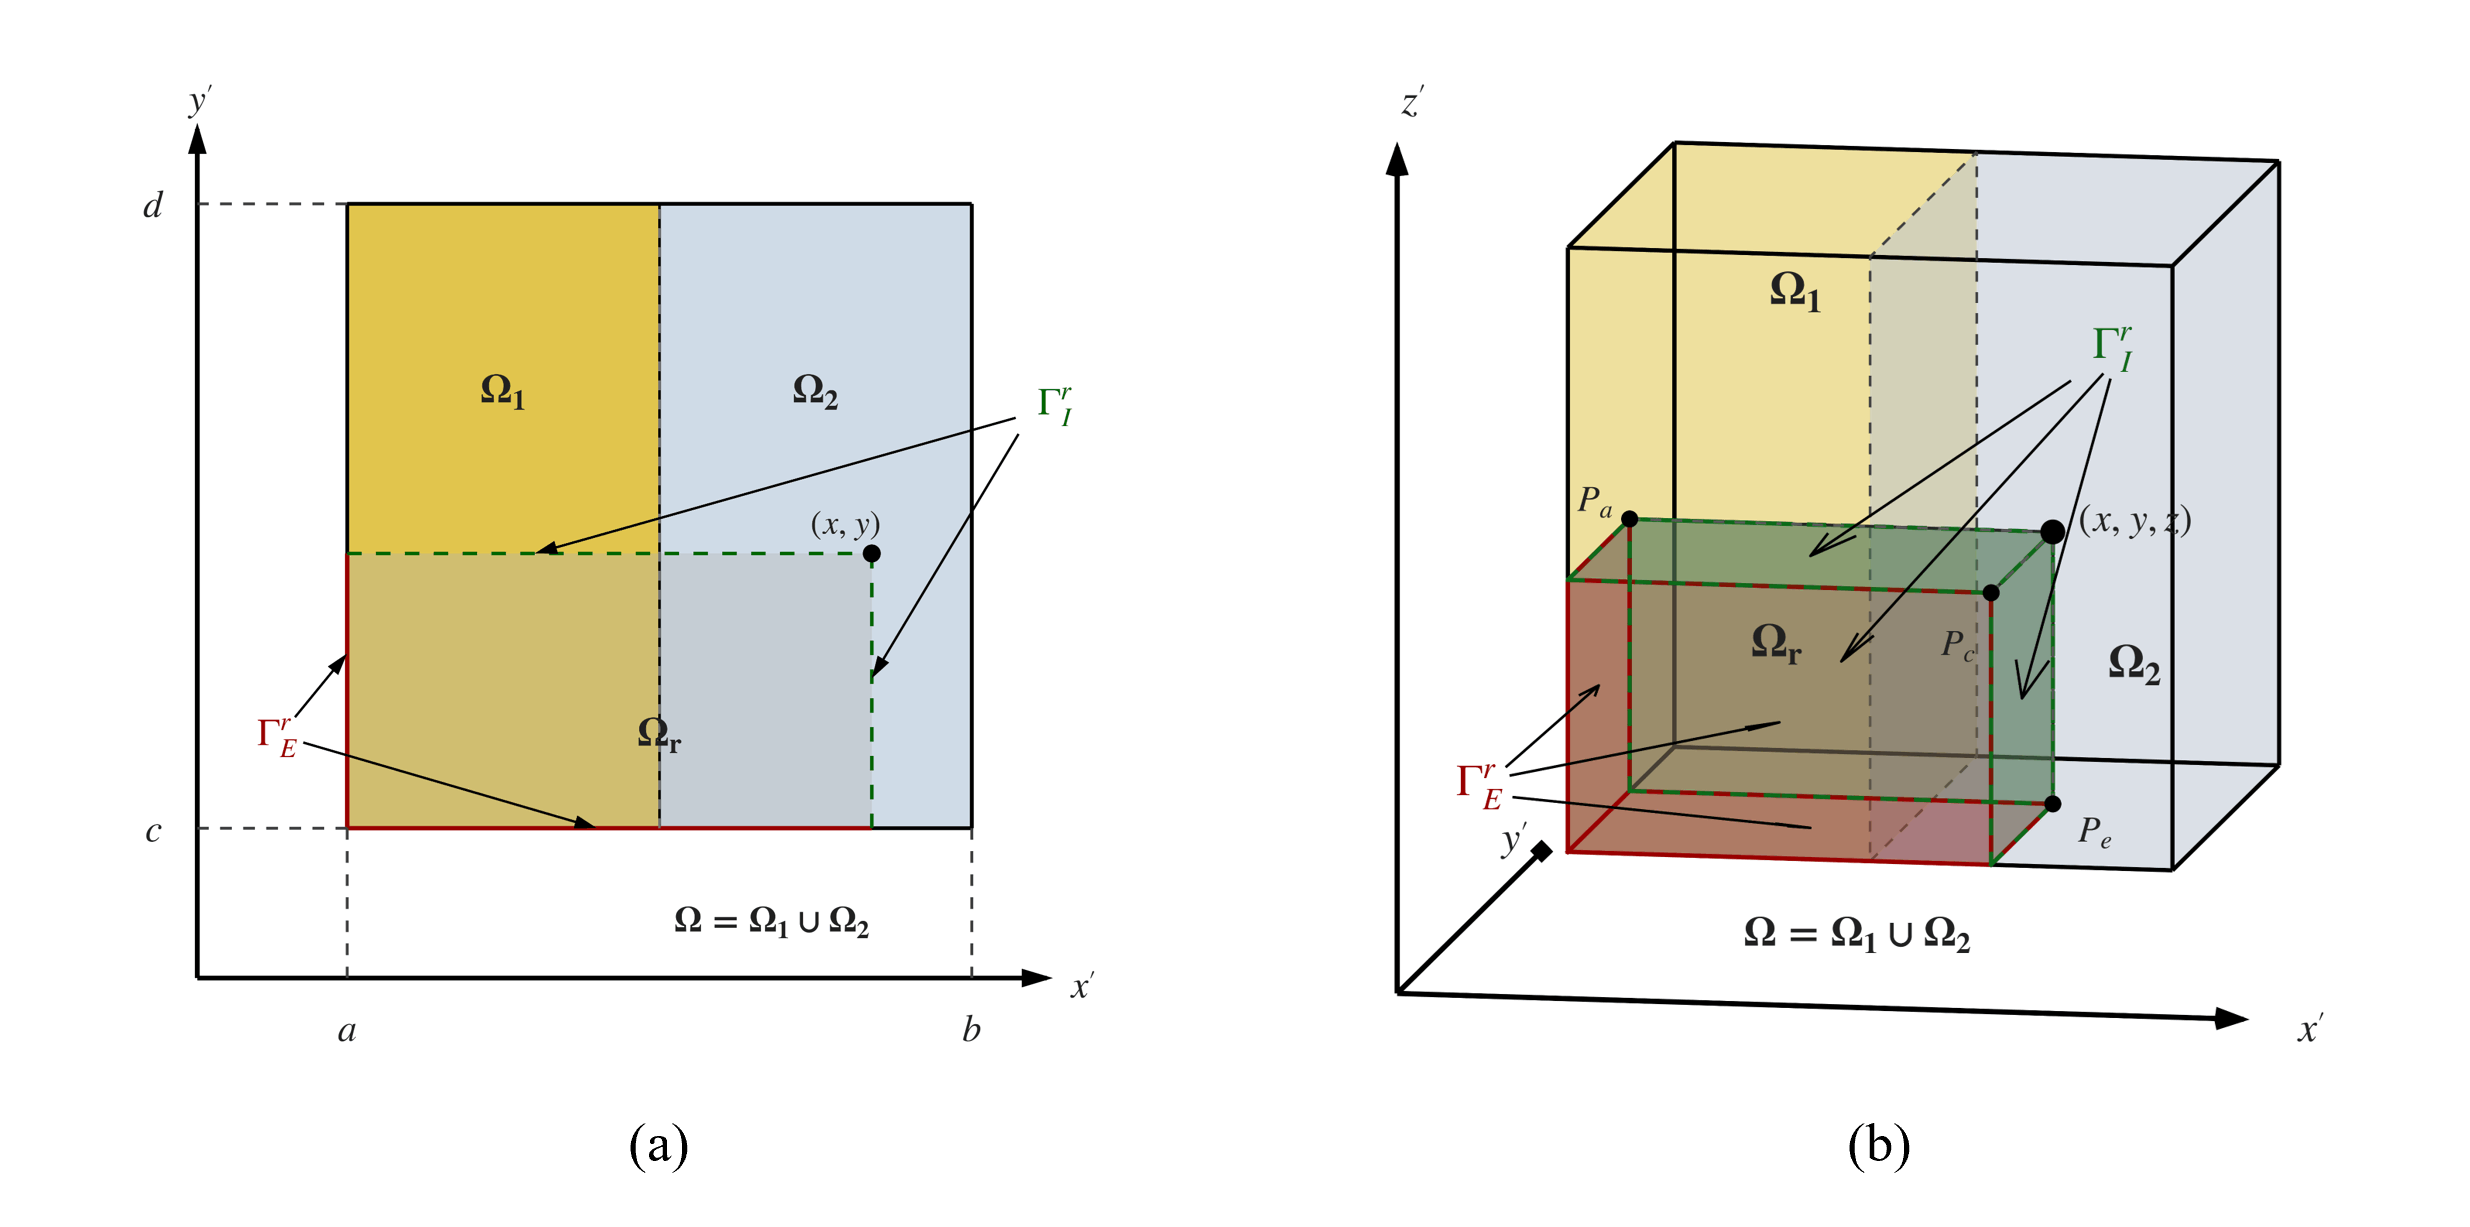
\includegraphics[width=0.72\textwidth]{./fig/figure_00.png}
    \caption{变域积分区域示意图：(a) 二维矩形区域；(b) 三维立方体区域。 }
    \label{fig:two_group_viws_g}
\end{figure}


以下通过第一群方程推导其弱形式。将 \cref{eq:two_group_eigenvalue} 中的首式在变域 $\Omega_{\boldsymbol r}$ 上积分，并选取常数测试函数 $v=1$，可得：
\begin{equation}
\begin{aligned}
    & \int_{c}^{y} \int_{a}^{x} \left[ -\nabla \cdot \left( D_1(x',y') \nabla \phi_1(x',y') \right) \right] \,dx'dy' \\
    &\quad + \int_{c}^{y} \int_{a}^{x} \left[ \Sigma_{\mathrm a,1}(x',y') + \Sigma_{\mathrm s,1\rightarrow2}(x',y') \right] \phi_1(x',y') \,dx'dy' \\
    &= \frac{1}{k_{\mathrm{eff}}} \int_{c}^{y} \int_{a}^{x} \left[ \nu_1\Sigma_{\mathrm f,1}(x',y')\phi_1(x',y') + \nu_2\Sigma_{\mathrm f,2}(x',y')\phi_2(x',y') \right] \,dx'dy' .
\end{aligned}
\label{eq:two_group_first_variable_integral}
\end{equation}
由于常数测试函数的梯度 $\nabla v$ 为零，同时利用基本弱解理论，上述扩散项可转化为边界积分形式：
\begin{equation}
\int_{c}^{y} \int_{a}^{x} \left[ -\nabla \cdot \left( D_1(x',y') \nabla \phi_1(x',y') \right) \right] dx'dy' = -\oint_{\partial\Omega_{\boldsymbol r}} D_1(x',y') \nabla \phi_1(x',y') \cdot \boldsymbol n d\gamma .
\label{eq:two_group_first_gauss_green}
\end{equation}

对于矩形子域 $\Omega_{\boldsymbol r}=[a,x]\times[c,y]$，其四条边界上的外法向量 $\boldsymbol n$ 分别为：$x'=a$ 处为 $(-1,0)$，$x'=x$ 处为 $(1,0)$，$y'=c$ 处为 $(0,-1)$，$y'=y$ 处为 $(0,1)$。据此，扩散项的边界积分可展开为：
\begin{equation}
\begin{aligned}
     -\oint_{\partial\Omega_{\boldsymbol r}} D_1(x',y') \nabla \phi_1(x',y') \cdot \boldsymbol n d\gamma
    &= \int_{c}^{y} D_1(a,y') \frac{\partial \phi_1}{\partial x'}(a,y') \,dy' - \int_{c}^{y} D_1(x,y') \frac{\partial \phi_1}{\partial x'}(x,y') \,dy' \\
    &\quad + \int_{a}^{x} D_1(x',c) \frac{\partial \phi_1}{\partial y'}(x',c) \,dx' - \int_{a}^{x} D_1(x',y) \frac{\partial \phi_1}{\partial y'}(x',y) \,dx' .
\end{aligned}
\label{eq:two_group_first_boundary_expand}
\end{equation}
将 \cref{eq:two_group_first_boundary_expand} 代入 \cref{eq:two_group_first_variable_integral}，即得第一群方程的二维变域积分弱形式。同理，对第二群方程在 $\Omega_{\boldsymbol r}$ 上积分并整理，可获得相应的弱形式方程。
因此，矩形区域上二维两群稳态扩散特征值问题的变域积分弱形式可写为
\begin{equation}
\left\{
\begin{aligned}
    &
    \int_{c}^{y}
    D_1(a,y')
    \frac{\partial \phi_1}{\partial x'}(a,y')
    \,dy'
    -
    \int_{c}^{y}
    D_1(x,y')
    \frac{\partial \phi_1}{\partial x'}(x,y')
    \,dy'
    \\
    &\quad
    +
    \int_{a}^{x}
    D_1(x',c)
    \frac{\partial \phi_1}{\partial y'}(x',c)
    \,dx'
    -
    \int_{a}^{x}
    D_1(x',y)
    \frac{\partial \phi_1}{\partial y'}(x',y)
    \,dx'
    \\
    &\quad
    +
    \int_{c}^{y}
    \int_{a}^{x}
    \left[
    \Sigma_{\mathrm a,1}(x',y')
    +
    \Sigma_{\mathrm s,1\rightarrow2}(x',y')
    \right]
    \phi_1(x',y')
    \,dx'dy'
    \\
    &=
    \frac{1}{k_{\mathrm{eff}}}
    \int_{c}^{y}
    \int_{a}^{x}
    \left[
    \nu_1\Sigma_{\mathrm f,1}(x',y')\phi_1(x',y')
    +
    \nu_2\Sigma_{\mathrm f,2}(x',y')\phi_2(x',y')
    \right]
    \,dx'dy',
    \\[0.8em]
    &
    \int_{c}^{y}
    D_2(a,y')
    \frac{\partial \phi_2}{\partial x'}(a,y')
    \,dy'
    -
    \int_{c}^{y}
    D_2(x,y')
    \frac{\partial \phi_2}{\partial x'}(x,y')
    \,dy'
    \\
    &\quad
    +
    \int_{a}^{x}
    D_2(x',c)
    \frac{\partial \phi_2}{\partial y'}(x',c)
    \,dx'
    -
    \int_{a}^{x}
    D_2(x',y)
    \frac{\partial \phi_2}{\partial y'}(x',y)
    \,dx'
    \\
    &\quad
    +
    \int_{c}^{y}
    \int_{a}^{x}
    \Sigma_{\mathrm a,2}(x',y')
    \phi_2(x',y')
    \,dx'dy'
    =
    \int_{c}^{y}
    \int_{a}^{x}
    \Sigma_{\mathrm s,1\rightarrow2}(x',y')
    \phi_1(x',y')
    \,dx'dy' .
\end{aligned}
\right.
\label{eq:two_group_variable_weak_form}
\end{equation}

针对三维问题，若 $\boldsymbol r=(x,y,z)$ 且计算域 $\Omega=[a,b]\times[c,d]\times[e,f]$，其变域积分区域定义为：
\begin{equation}
    \Omega_{\boldsymbol r} = [a,x]\times[c,y]\times[e,z].
    \label{eq:two_group_variable_domain_3d}
\end{equation}
其原理如图 \cref{fig:two_group_viws_g}(b) 所示。三维情形的推导思路与二维类似，主要区别在于变域边界由线段扩展为曲面，相应边界积分也由线积分变为空间曲面积分。此外，该方法可直接推广至其余多群扩散方程组。



%====================================================
\subsection{原函数变换}
\label{subsec:antiderivative_transform}
{\color{black}
在构建 \cref{eq:multigroup_variable_weak_form} 所示的变域积分弱形式后，若直接采用传统数值积分方法处理其中的变域积分项，由于深度学习方法涉及大规模迭代优化，密集的离散求和计算将导致显著的计算负载 \cite{liu2025neutron, guan2022solving, sun2023binn, guo2022physics}。为提升计算效率，本文引入原函数变换理论 \cite{LiuDong2025DuoWeiLian}，旨在将满足连续性条件的变域积分项转化为等价的局部微分约束，从而降低待处理数值积分项的规模。

针对 \cref{eq:multigroup_variable_weak_form} 中的扩散体积分项，若被积函数 $D_g(\boldsymbol \xi) \nabla \phi_g(\boldsymbol \xi) \cdot \nabla v(\boldsymbol \xi)$ 在积分域内连续，根据 Newton--Leibniz 公式 \cite{courant1999introduction} 及相关理论 \cite{LiuDong2025DuoWeiLian}，可定义原函数 $F_{g,0}(\boldsymbol r)$ 使其满足如下微分-积分关系：
\begin{equation}
    \left\{
    \begin{aligned}
        F_{g,0}(\boldsymbol r) &= \int_{\Omega_{\boldsymbol r}} D_g(\boldsymbol \xi) \nabla \phi_g(\boldsymbol \xi) \cdot \nabla v(\boldsymbol \xi) \,d\boldsymbol \xi , \\
        \frac{\partial^d F_{g,0}}{\partial r_1\partial r_2\cdots\partial r_d} &= D_g(\boldsymbol r) \nabla \phi_g(\boldsymbol r) \cdot \nabla v(\boldsymbol r) .
    \end{aligned}
    \right.
    \label{eq:Fg0_integral}
\end{equation}
由于原函数族在定义上相差一个关于 $\boldsymbol{r}$ 的函数项 $C(\boldsymbol{r})$ \cite{courant1999introduction}，为保证其唯一性，必须引入特定的定解条件，记为 $F_{g,0}({\boldsymbol{r}}_{a}) = {g}_{a}$。关于这类定解条件的构造及其具体讨论，可参见文献 \cite{LiuDong2025DuoWeiLian, LiuDong2025MianXiangShen, LiuDong2026MianXiangShen}。

同理，对于 \cref{eq:multigroup_variable_weak_form} 中的边界积分项，若被积函数 $\left[ -D_g(\boldsymbol \xi) \nabla \phi_g(\boldsymbol \xi) \cdot \boldsymbol n \right] v(\boldsymbol \xi)$ 满足连续性要求，可将其沿坐标方向进行分解。在满足定解约束 $F_{g,\ell}(\boldsymbol r_b) = {g}_{\ell}$ 的前提下，可确定第 $\ell$ 个坐标方向对应的原函数 $F_{g,\ell}(\boldsymbol r)$。通过上述变换，原变域积分弱形式 \cref{eq:multigroup_variable_weak_form} 最终可转化为如下变阶弱形式：
\begin{equation}
    \begin{aligned}
    & F_{g,0}(\boldsymbol r) - \sum_{\ell=1}^{d}F_{g,\ell}(\boldsymbol r) + \int_{\Omega_{\boldsymbol r}} \Sigma_{t,g}(\boldsymbol \xi) \phi_g(\boldsymbol \xi) v(\boldsymbol \xi) \,d\boldsymbol \xi \\
    \quad & =
    \int_{\Omega_{\boldsymbol r}}
    \left[
    \sum_{g'=1}^{G}
    \Sigma_{\mathrm{s},g'\to g}(\boldsymbol \xi)
    \phi_{g'}(\boldsymbol \xi)
    +
    \frac{\chi_g}{k_{\mathrm{eff}}}
    \sum_{g'=1}^{G}
    \left(\nu\Sigma_{\mathrm{f}}\right)_{g'}(\boldsymbol \xi)
    \phi_{g'}(\boldsymbol \xi)
    \right]
    v(\boldsymbol \xi)\,d\boldsymbol \xi ,
    \qquad g=1,2,\ldots,G .
    \end{aligned}
    \label{eq:variable_order_mg_main}
\end{equation}
}

{\color{black}
%====================================================
\subsection{变阶弱形式的深度学习求解}
\label{sec:nn_loss}

在获得 \cref{eq:variable_order_mg_main} 所示的变阶形式后，可基于经典 PINN 架构 \cite{raissi2019physicsinformed} 或改进的微分方程深度学习框架 \cite{lu2021deepxde, sengupta2020review, wang2024multistage} 进行求解。本文采用神经网络近似各能群中子通量及相应原函数。对于第 $g$ 个能群，中子通量表示为
\begin{equation}
    \phi_{g,\theta}(\boldsymbol r)
    =
    \mathcal{N}_{\phi_g}(\boldsymbol r;\theta_g),
    \qquad g=1,2,\ldots,G ,
    \label{eq:nn_phi_g}
\end{equation}
其中，$\mathcal{N}_{\phi_g}$ 为第 $g$ 群中子通量网络，$\theta_g$ 为其网络参数。

类似地，原函数项可表示为
\begin{equation}
    F_{g,m,\eta}(\boldsymbol r)
    =
    \mathcal{N}_{F_{g,m}}(\boldsymbol r;\eta_{g,m}),
    \qquad
    m=0,1,\ldots,d .
    \label{eq:nn_F_g}
\end{equation}
其中，$F_{g,0,\eta}$ 对应扩散体积分项的原函数，$F_{g,\ell,\eta}$ 对应第 $\ell$ 个坐标方向的边界通量原函数，$\ell=1,2,\ldots,d$。实际实现中，可为不同原函数分别构造独立网络，也可采用多输出神经网络统一表示多个原函数分量。

基于上述近似，总损失函数由主方程残差、原函数定义约束、原函数定解条件和物理边界条件组成：
\begin{equation}
    \mathcal{L}
    =
    w_{\mathrm r}\mathcal{L}_{\mathrm r}
    +
    w_{\mathrm{def}}\mathcal{L}_{\mathrm{def}}
    +
    w_F\mathcal{L}_{F}
    +
    w_{\mathrm b}\mathcal{L}_{\mathrm b},
    \label{eq:total_loss_viws}
\end{equation}
其中，$\mathcal{L}_{\mathrm r}$ 用于约束 \cref{eq:variable_order_mg_main} 所示的主方程残差；$\mathcal{L}_{\mathrm{def}}$ 用于约束原函数与其对应被积函数之间的微分关系；$\mathcal{L}_{F}$ 用于施加原函数定解条件；$\mathcal{L}_{\mathrm b}$ 用于满足 \cref{eq:mg_bc} 所示的物理边界条件。$w_{\mathrm r}$、$w_{\mathrm{def}}$、$w_F$ 和 $w_{\mathrm b}$ 为相应损失权重。

需要说明的是，\cref{eq:variable_order_mg_main} 中满足连续性要求的扩散体积分项和部分边界通量项通过原函数网络及其自动微分进行约束；而吸收项、散射项和裂变源项通常包含材料相关宏观截面，在多材料问题中可能存在界面跳变，因此通过数值积分进行计算。这样既减少了需要直接数值积分的项数，又避免了对不连续项强行构造全域原函数。

训练过程中，通过优化所有神经网络参数，使总损失函数 \cref{eq:total_loss_viws} 逐步减小。当损失值达到预设精度要求或满足停止准则时，$\mathcal{N}_{\phi_g}(\boldsymbol r;\theta_g)$ 即作为第 $g$ 群中子通量 $\phi_g(\boldsymbol r)$ 的数值近似。相关实现细节可参见 \cite{liu2025neutron, LiuDong2025DuoWeiLian}。
}

\section{数值实验}
\label{sec:numerical_experiments}

本节通过五个算例验证 VIWS 方法求解不连续系数中子扩散方程的能力，覆盖二维复杂边界、三维多界面结构、圆柱棒束阵列、两群固定源问题和 2D-IAEA 两群特征值基准题。参考解均由高精度有限元方法（FEM）获得，对比方法采用标准 PINN~\cite{raissi2019physicsinformed}。

除特别说明外，各算例采用相同训练设置。损失函数中各项权重 $w_{\mathrm r}$、$w_{\mathrm{def}}$、$w_F$ 和 $w_{\mathrm b}$ 根据各约束项的物理含义和数值实验经验选取。训练采用 Adam 与 L-BFGS 结合的两阶段策略：Adam 阶段学习率为 $10^{-3}$，迭代 $2000$ 步；随后采用 L-BFGS 进一步优化，直至损失函数满足收敛准则。默认网络为 8 层全连接神经网络，每层 32 个神经元，激活函数为 Tanh。


预测精度采用相对 $L_2$ 误差衡量：
\begin{equation}
    \label{eq:l2_error}
    \epsilon_{L_2}
    =
    \frac{\|\hat{\phi}-\phi_{\mathrm{ref}}\|_2}{\|\phi_{\mathrm{ref}}\|_2}
    =
    \sqrt{
        \frac{
            \sum_{i=1}^{N}
            \left(
            \hat{\phi}(\boldsymbol r_i)-\phi_{\mathrm{ref}}(\boldsymbol r_i)
            \right)^2
        }{
            \sum_{i=1}^{N}
            \phi_{\mathrm{ref}}^2(\boldsymbol r_i)
        }},
\end{equation}
其中 $\hat{\phi}$ 为神经网络预测通量，$\phi_{\mathrm{ref}}$ 为 FEM 参考通量，$N$ 为测试点数量。对于特征值问题，有效增殖因子偏差采用 pcm 表示，即
$\Delta k_{\mathrm{pcm}}=|k_{\mathrm{NN}}-k_{\mathrm{ref}}|\times 10^5$。
%=============================================================
\subsection{算例 1：2D 正六边形单群固定源问题}
\label{subsec:case1}

本算例考虑二维正六边形区域中的单群固定源问题，用于考察 VIWS 在复杂外边界问题上的性能。\cref{eq:multigroup_fixed_source} 对应的单群固定源方程形式为
{\color{black}
\begin{equation}
-\nabla\cdot \left( D(\boldsymbol r)\nabla\phi(\boldsymbol r) \right) + \Sigma_{\mathrm{t}}(\boldsymbol r)\phi(\boldsymbol r) = \nu\Sigma_{\mathrm{f}}(\boldsymbol r)\phi(\boldsymbol r) + S(\boldsymbol r), \quad \boldsymbol r\in\Omega
\label{eq:single_group_diffusion}
\end{equation}}
其中 $\boldsymbol r=(x,y)$，$\phi$ 为单群中子通量。外边界施加齐次 Dirichlet 条件：
$\phi(\boldsymbol r)=0,\ \boldsymbol r\in\partial\Omega$。

计算域 $\Omega$ 为外接圆半径 $R=1.0\,\mathrm{cm}$ 的正六边形，并由两个同心圆界面划分为三个子域 $\Omega_1$、$\Omega_2$ 和 $\Omega_3$。\cref{fig:case1_geometry_reference_testfunction}(a) 给出几何与材料分区，\cref{fig:case1_geometry_reference_testfunction}(b) 给出 FEM 参考通量。材料参数列于~\cref{tab:case1_material_parameters}。

\begin{table}[H]{\color{black}
    \centering
    \caption{算例 1：2D 正六边形单群固定源问题的材料参数}
    \label{tab:case1_material_parameters}
    % \small
    \begin{tabularx}{0.95\textwidth}{@{\extracolsep{\fill}}cccccc}
        \toprule
        子域         & 径向范围               & $D$\,(cm) & $\Sigma_{\mathrm{t}}$\,(cm$^{-1}$) & $\nu\Sigma_{\mathrm{f}}$\,(cm$^{-1}$) & $S$ (cm$^{-3}\cdot$s$^{-1}$) \\
        \midrule
        $\Omega_1$ & $r \le 0.5$        & 1.00      & 0.220                              & 0.120                                 & 10                       \\
        $\Omega_2$ & $0.5 < r \le 0.65$ & 0.25      & 0.060                              & 0.000                                 & 0                        \\
        $\Omega_3$ & $r > 0.65$         & 4.00      & 0.020                              & 0.000                                 & 0                        \\
        \bottomrule
    \end{tabularx}}
\end{table}
VIWS 采用四个相互独立的神经网络分别表示中子通量 $\phi(x,y)$ 和原函数 $\{F_k\}_{k=0}^{2}$，域内与边界采样点总数为 $10,000$。针对正六边形边界，本文采用在 $\partial\Omega$ 上为零的钟形神经网络测试函数，其空间分布见~\cref{fig:case1_geometry_reference_testfunction}(c)。

\begin{figure}[H]
    \centering
    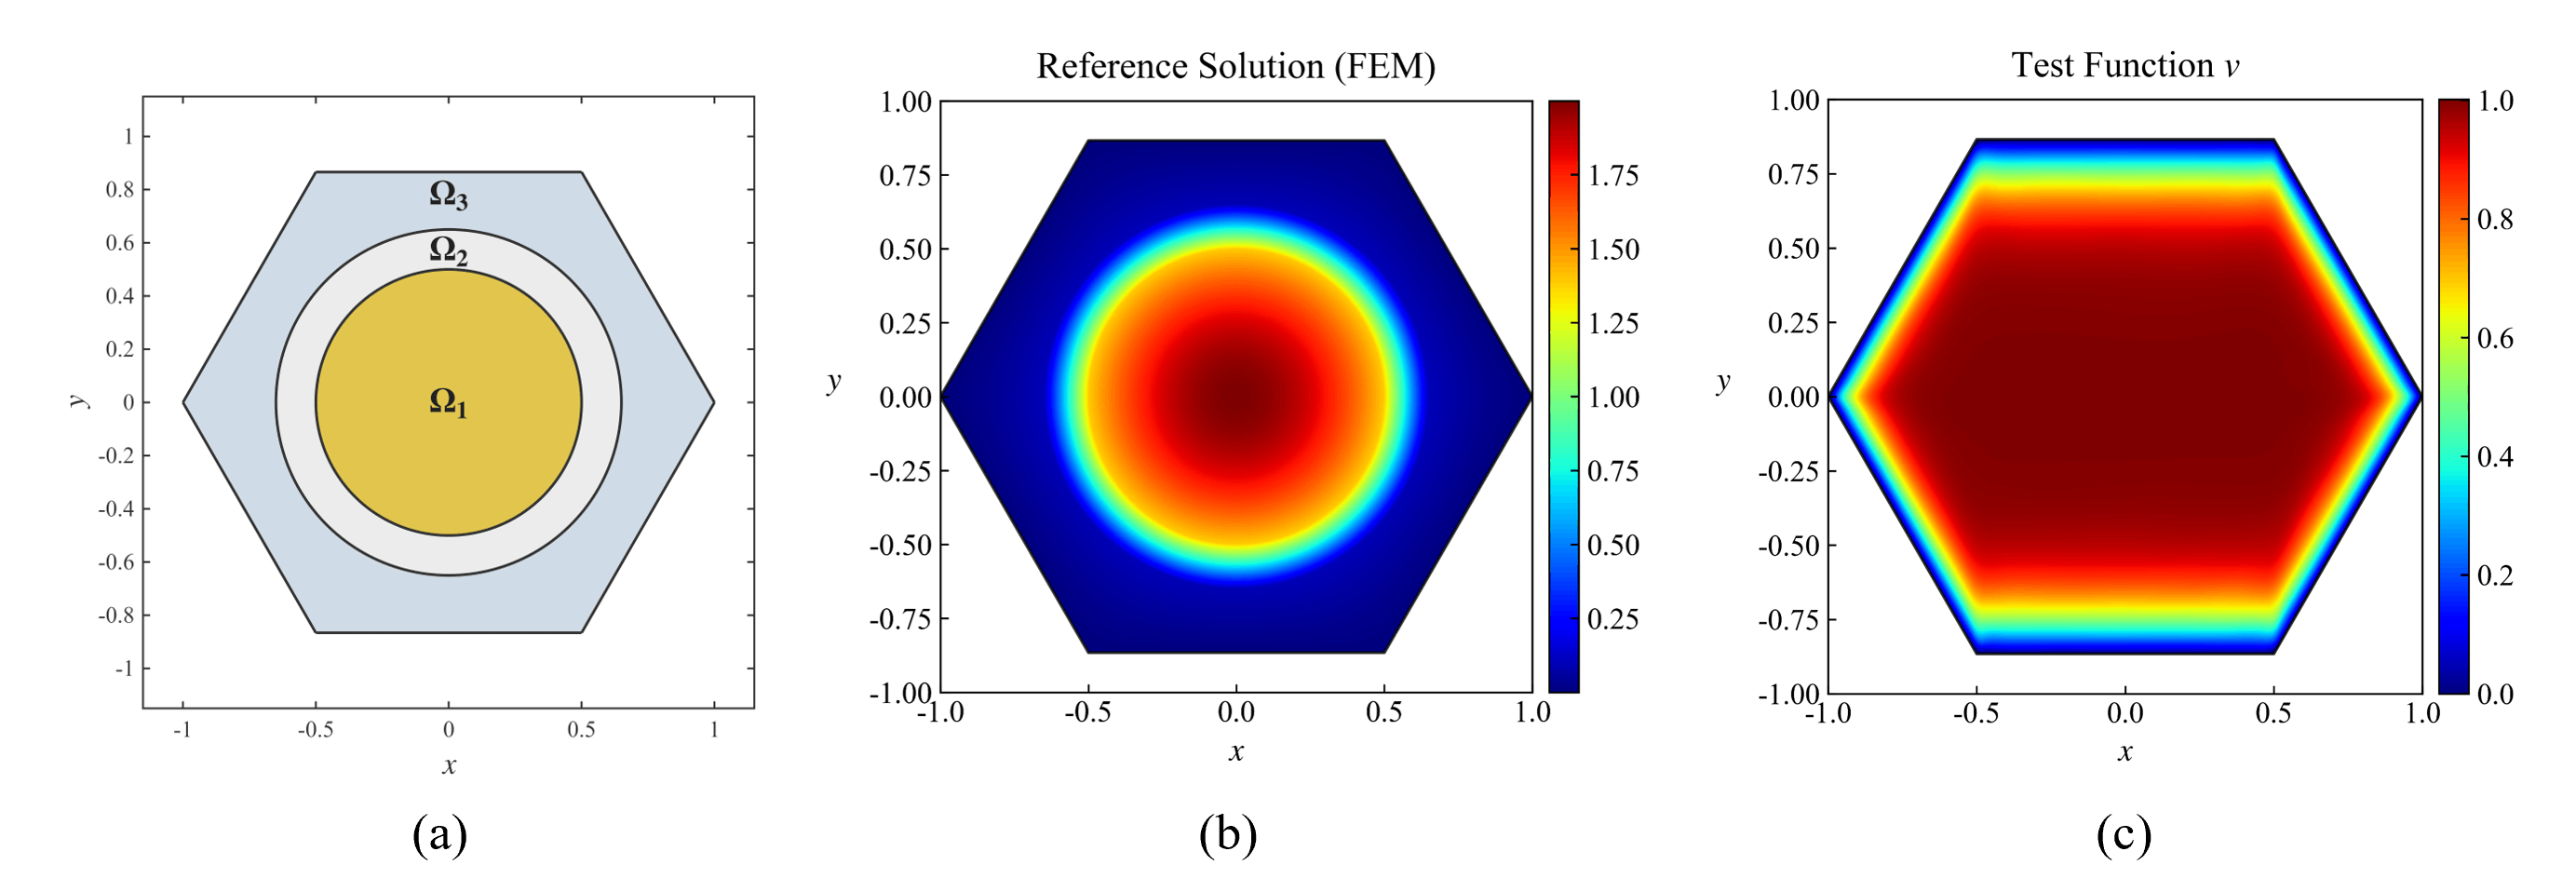
\includegraphics[width=0.85\textwidth]{fig/figure_01.png}
    \caption{算例 1：2D 正六边形单群固定源问题的计算设置。(a) 几何与材料分区；(b) FEM 参考通量；(c) 神经网络测试函数 $v$。}
    \label{fig:case1_geometry_reference_testfunction}
\end{figure}

~\cref{fig:case1_flux_error_comparison} 比较了标准 PINN 与 VIWS 的通量预测结果及绝对误差。标准 PINN 的相对 $L_2$ 误差为 $4.04\times10^{-1}$，误差主要集中在源区 $\Omega_1$ 附近；VIWS 的相对 $L_2$ 误差降至 $1.25\times10^{-2}$。\cref{fig:case1_antiderivative_fields} 给出了 VIWS 学习得到的原函数场 $F_0$、$F_1$ 和 $F_2$。{\color{black}结果表明，VIWS 在处理复杂外边界问题上具有良好适用性,其精度相较于 PINN 具有明显提升。}

\begin{figure}[H]
    \centering
    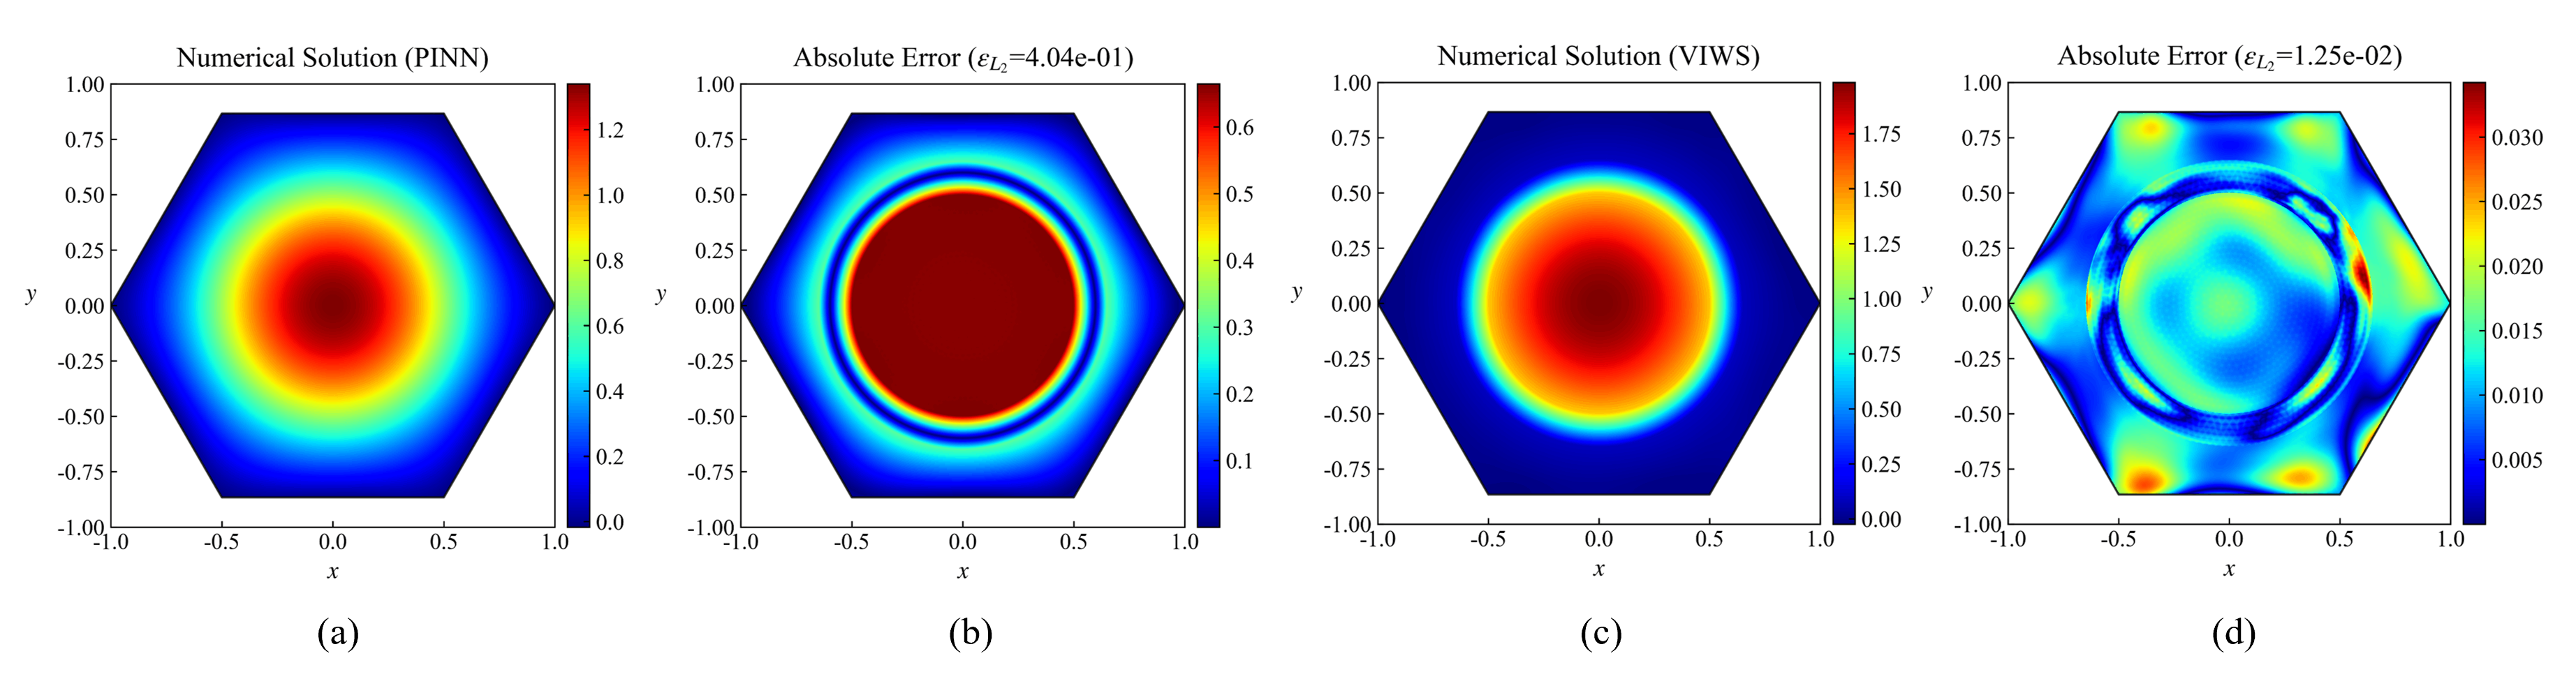
\includegraphics[width=1\textwidth]{fig/figure_02.png}
    \caption{算例 1：2D 正六边形单群固定源问题的通量预测与误差对比。(a) PINN 预测通量；(b) PINN 绝对误差；(c) VIWS 预测通量；(d) VIWS 绝对误差。}
    \label{fig:case1_flux_error_comparison}
\end{figure}

\begin{figure}[H]
    \centering
    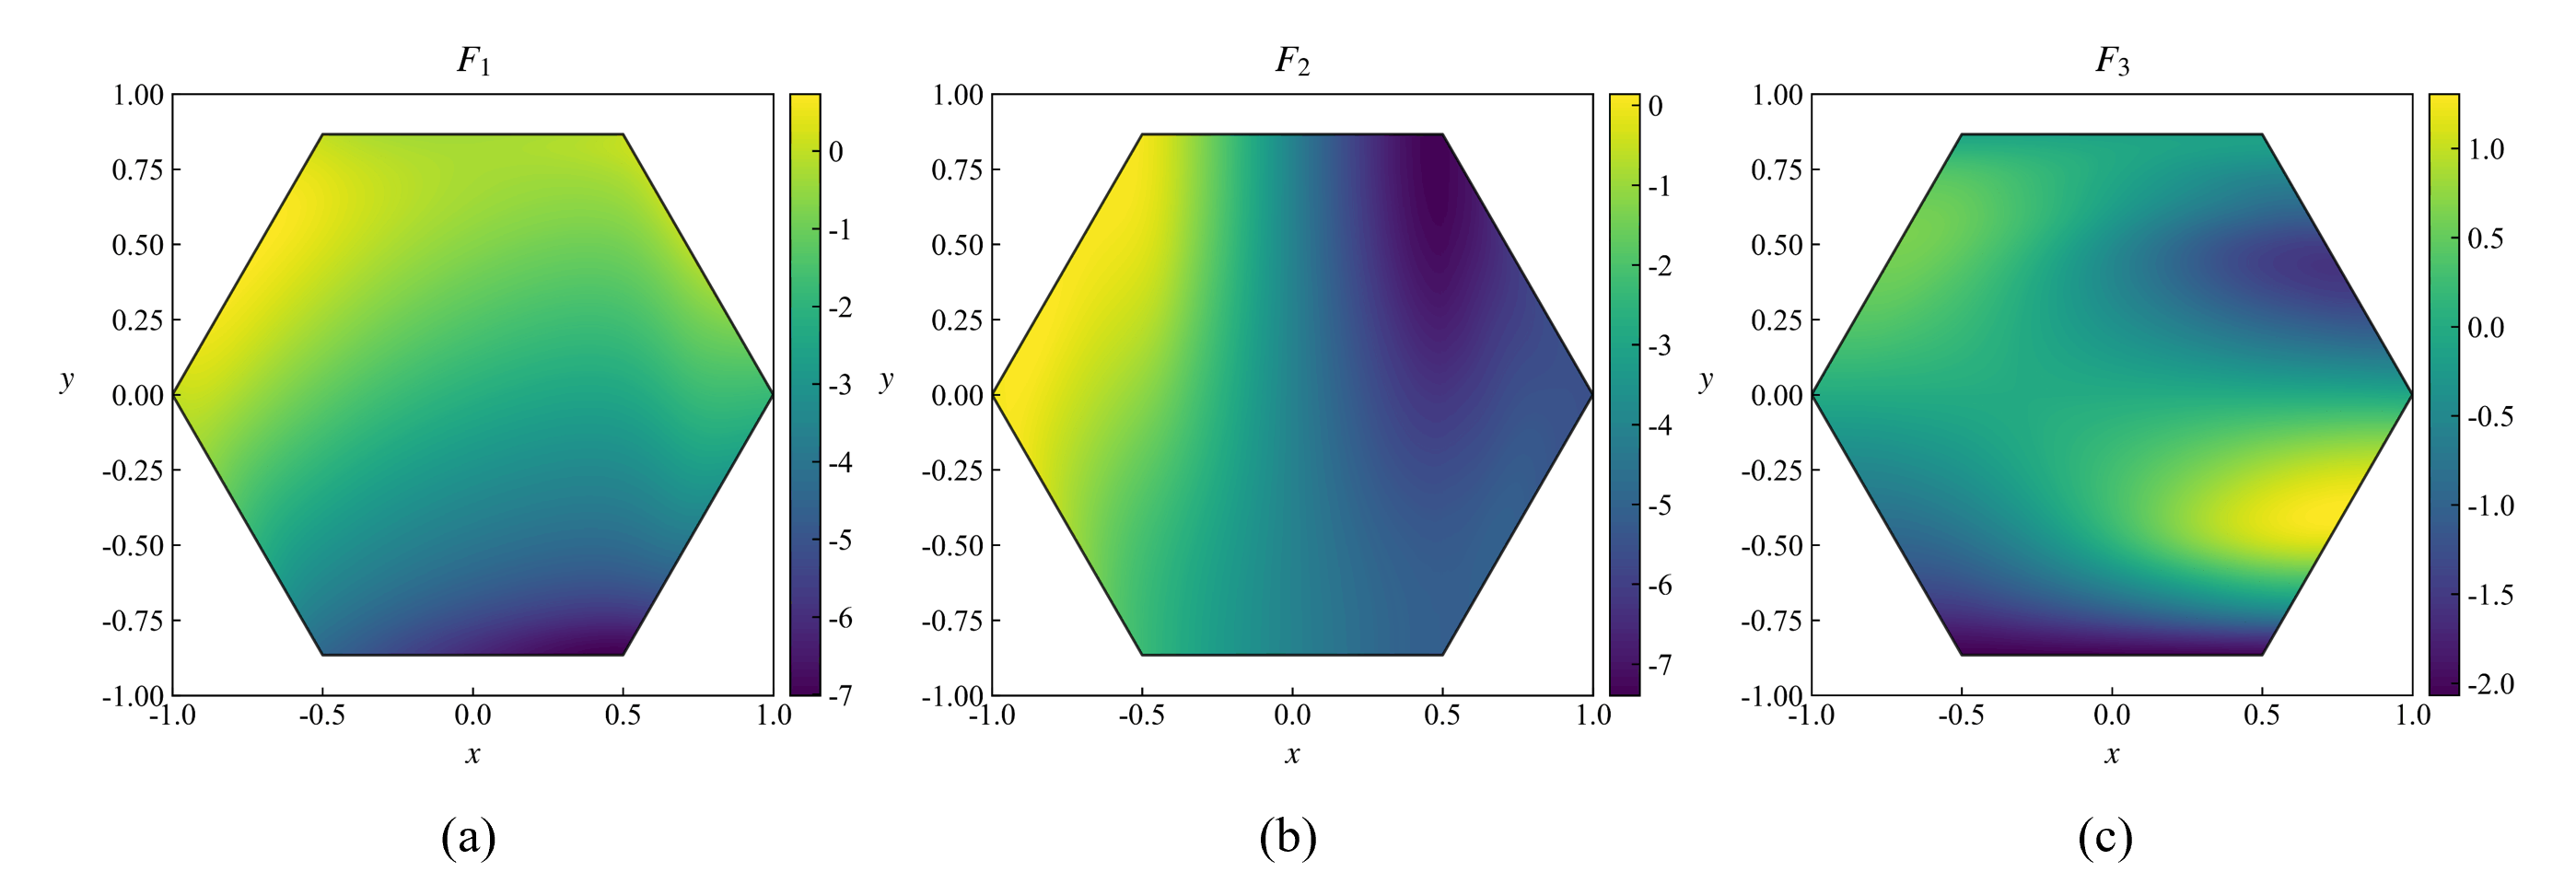
\includegraphics[width=0.75\textwidth]{fig/figure_03.png}
    \caption{算例 1：2D 正六边形三材料单群固定源问题的原函数场。(a) $F_0$；(b) $F_1$；(c) $F_2$。}
    \label{fig:case1_antiderivative_fields}
\end{figure}

%=============================================================
\subsection{算例 2：3D 八区域单群固定源问题}
\label{subsec:case2}

本算例考察 VIWS 在三维多界面非均匀介质问题中的性能。控制方程仍采用~\cref{eq:single_group_diffusion}，其中 $\boldsymbol r=(x,y,z)$，外边界施加齐次 Dirichlet 条件。

计算域为 $\Omega=[-1,1]^3$。三个坐标平面将立方体划分为 8 个子区域 $\Omega_1,\ldots,\Omega_8$。\cref{fig:case2_geometry_reference}(a) 给出几何与材料分区，\cref{fig:case2_geometry_reference}(b) 给出 FEM 参考通量。材料参数列于~\cref{tab:case2_material_parameters}。

\begin{table}[H]{\color{black}
    \centering
    \caption{算例 2：3D 八区域单群固定源问题的材料参数}
    \label{tab:case2_material_parameters}
    % \small
    \begin{tabularx}{0.95\textwidth}{@{\extracolsep{\fill}}ccccc}
        \toprule
        子域                                       & $D$ (cm) & $\Sigma_{\mathrm{t}}$ (cm$^{-1}$) & $\nu\Sigma_{\mathrm{f}}$ (cm$^{-1}$) & $S$ (cm$^{-3}\cdot$s$^{-1}$) \\
        \midrule
        $\Omega_1, \Omega_3, \Omega_6, \Omega_8$ & 1.00     & 0.220                             & 0.120                                & 10.0                    \\
        $\Omega_2, \Omega_4, \Omega_5, \Omega_7$ & 4.00     & 0.020                             & 0.000                                & 0.0                     \\
        \bottomrule
    \end{tabularx}}
\end{table}

\begin{figure}[H]
    \centering
    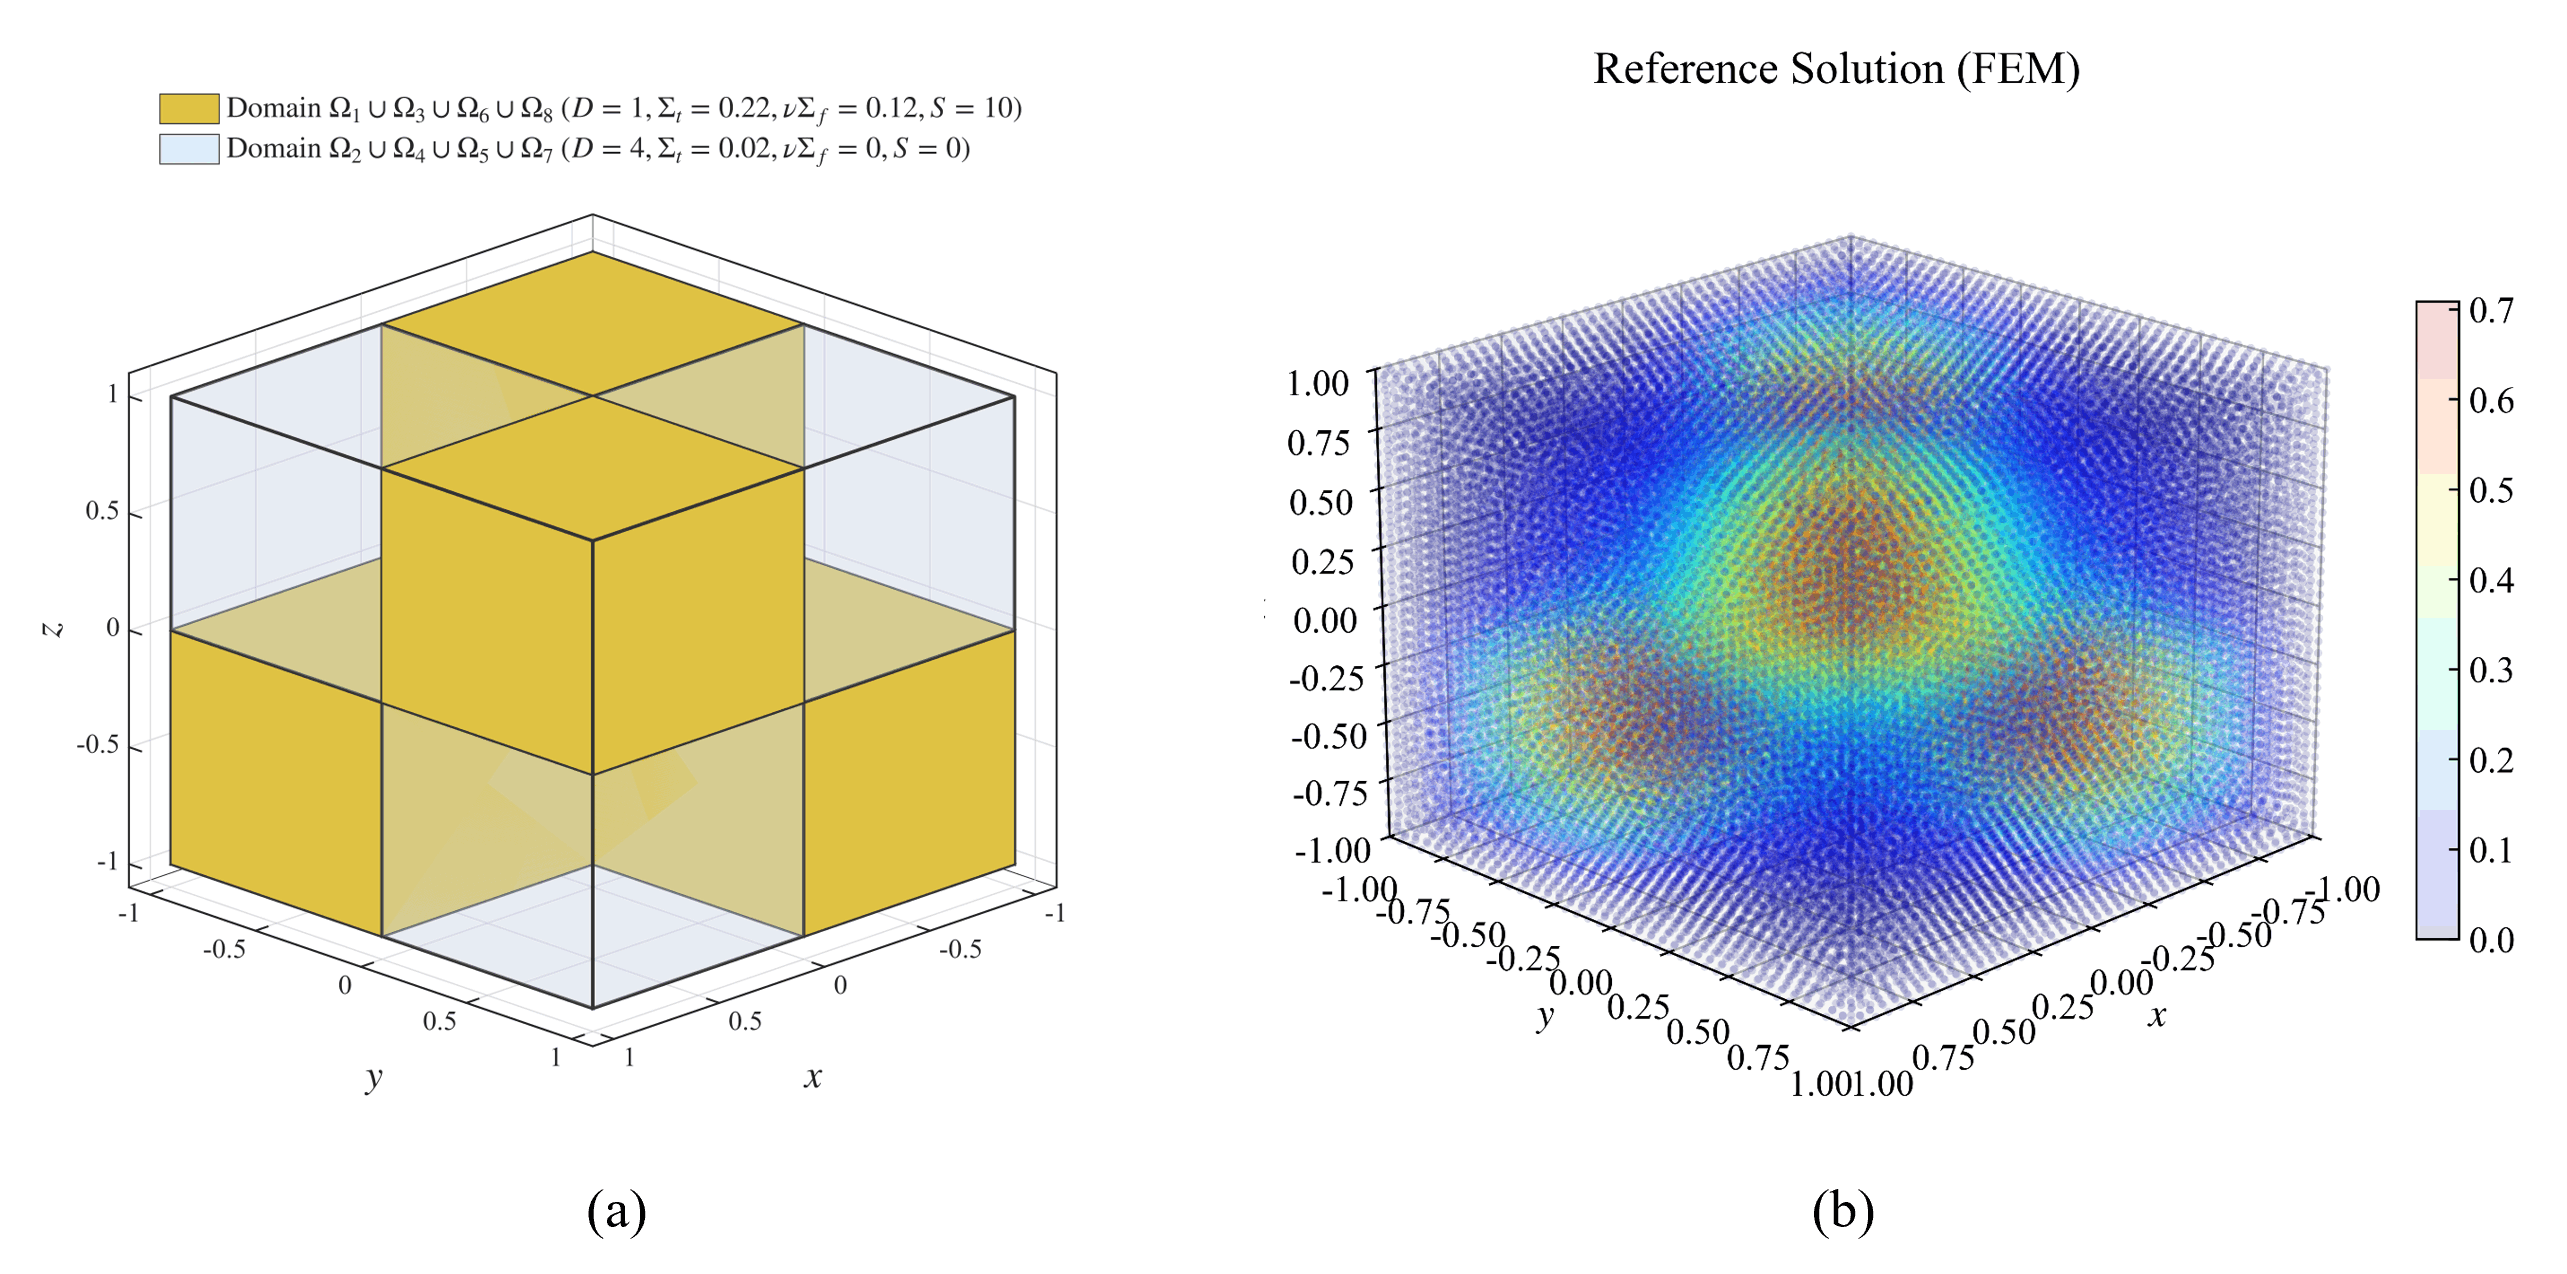
\includegraphics[width=0.7\textwidth]{fig/figure_04.png}
    \caption{算例 2：3D 八区域单群固定源问题的计算设置。(a) 几何与材料分区；(b) FEM 参考通量。}
    \label{fig:case2_geometry_reference}
\end{figure}

本算例选取在部分边界上为零的测试函数
$v=(x+1)(y+1)(z+1)$，并采用五个独立神经网络分别表示 $\phi(x,y,z)$ 和 $\{F_k\}_{k=0}^{3}$，采样点数为 $216,000$。

~\cref{fig:case2_flux_error_comparison} 显示了标准 PINN 与 VIWS 的通量预测和误差分布。标准 PINN 在内部界面及界面交汇区域产生明显误差，相对 $L_2$ 误差为 $3.20\times10^{-1}$；VIWS 的相对 $L_2$ 误差为 $2.60\times10^{-2}$。\cref{fig:case2_antiderivative_fields} 给出了 VIWS 对应的原函数 $F_0$、$F_1$、$F_2$ 和 $F_3$。{\color{black}结果说明，本文所提方法能够较好处理高维非均匀介质界面引起的通量梯度不连续问题。相对于经典PINN方法仍然具有明显精度优势。鉴于这种基于规则三维节块的扩散计算在大型反应堆堆芯工程设计与分析中较为常见\cite{liu2024deep}，本算例也从工程应用角度验证了该方法处理三维多界面问题的适用性。}

\begin{figure}[H]
    \centering
    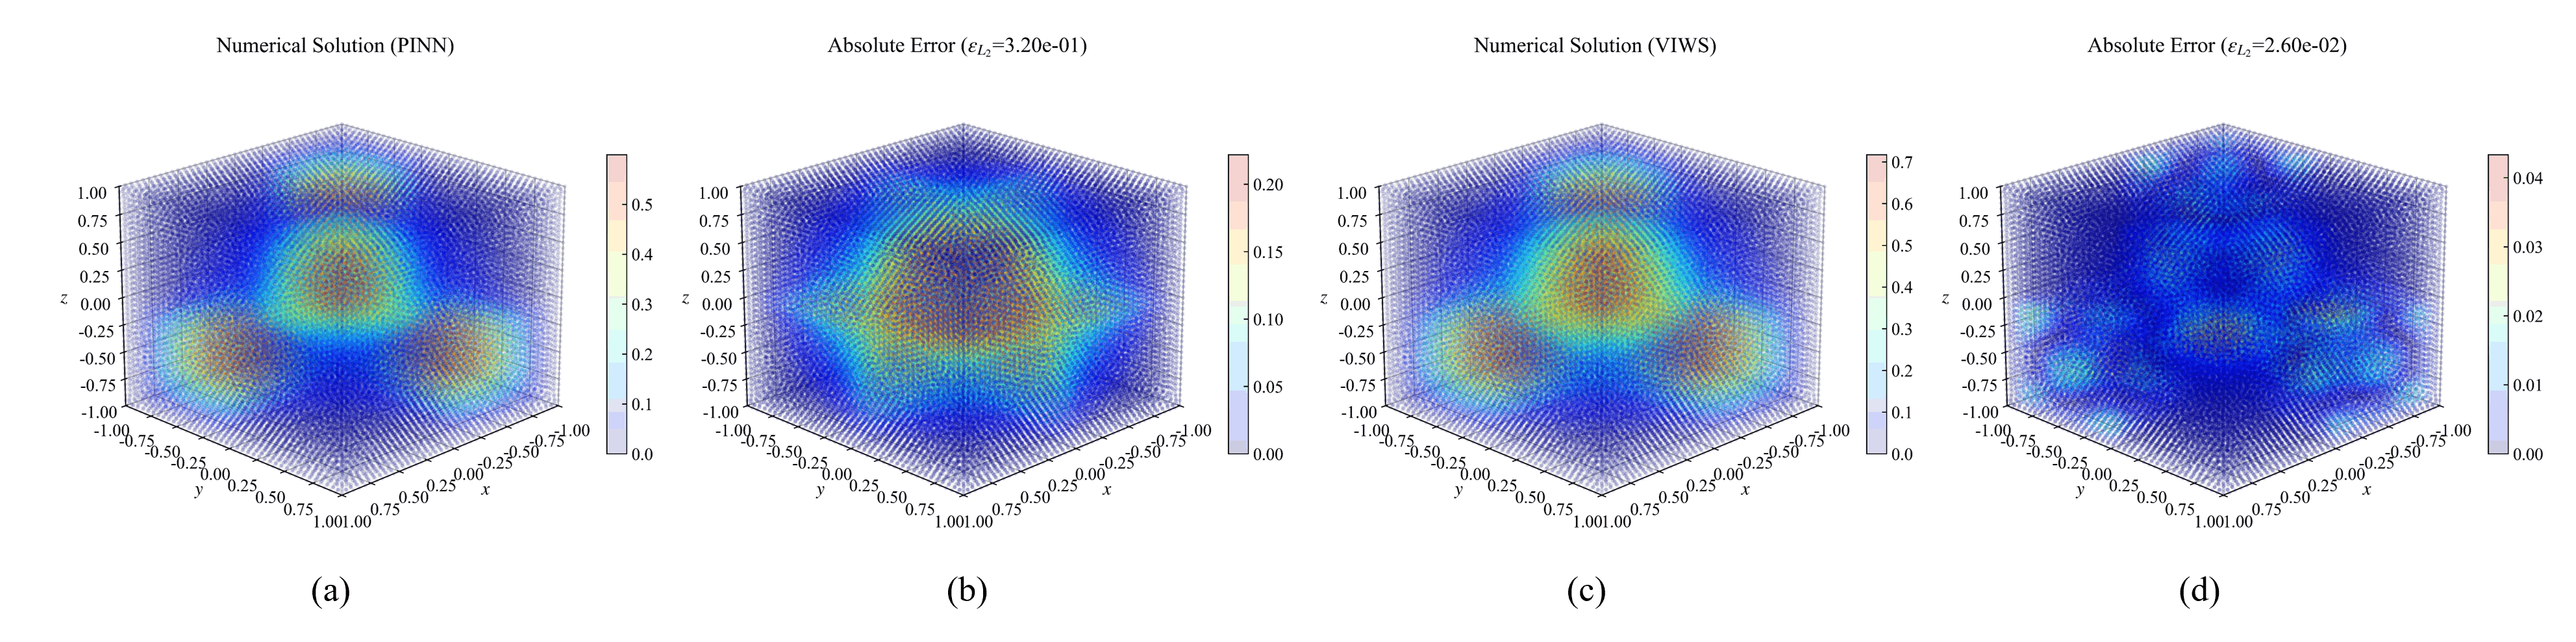
\includegraphics[width=1\textwidth]{fig/figure_05.png}
    \caption{算例 2：3D 八区域单群固定源问题的通量预测与误差对比。(a) PINN 预测通量；(b) PINN 绝对误差；(c) VIWS 预测通量；(d) VIWS 绝对误差。}
    \label{fig:case2_flux_error_comparison}
\end{figure}

\begin{figure}[H]
    \centering
    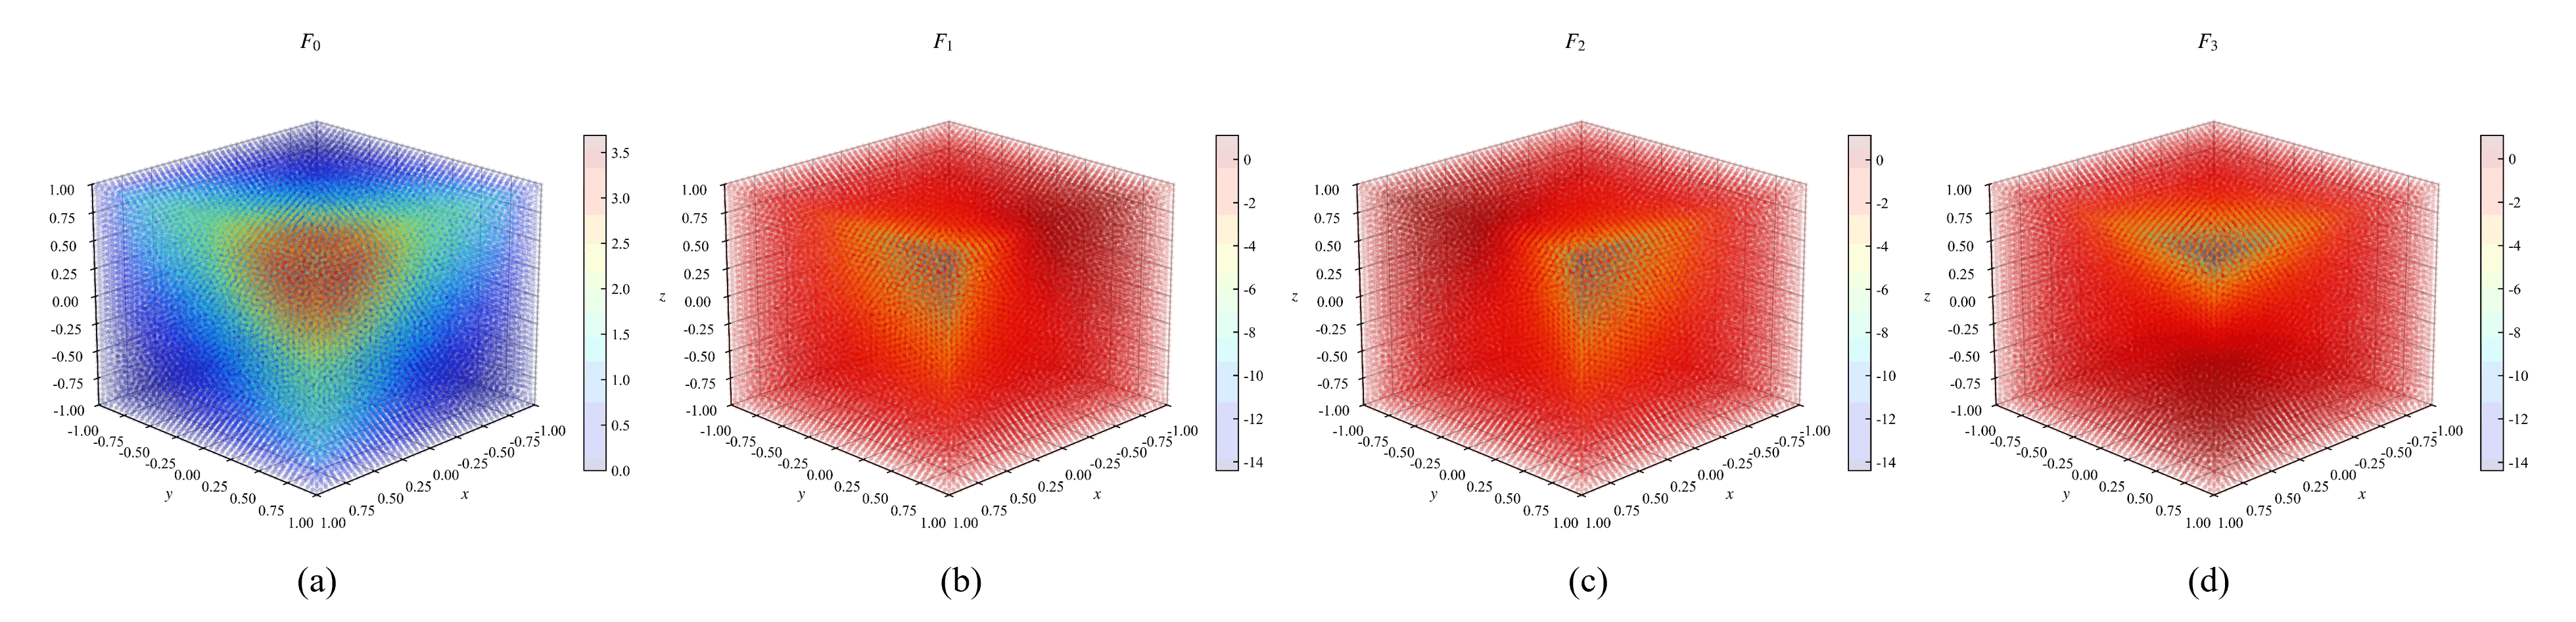
\includegraphics[width=1\textwidth]{fig/figure_06.png}
    \caption{算例 2：3D 八区域单群固定源问题的原函数场。(a) $F_0$；(b) $F_1$；(c) $F_2$；(d) $F_3$。}
    \label{fig:case2_antiderivative_fields}
\end{figure}

%=============================================================
\subsection{算例 3：3D 圆柱棒束阵列单群固定源问题} \label{subsec:case3}

本算例通过模拟纵向贯穿的圆柱棒束阵列，进一步验证 VIWS 方法在处理多曲面几何界面及混合边界条件时的适用性。控制方程采用~\cref{eq:single_group_diffusion}，其中空间位置记为 $\boldsymbol r=(x,y,z)$。
计算域设定为立方体区域 $\Omega=[-1,1]^3$。为模拟典型的堆芯物理边界，侧边界施加齐次 Dirichlet 条件（$\phi=0$）；上、下端面（$z=\pm1$）则施加零法向梯度的 Neumann 条件，即 $\nabla\phi \cdot \boldsymbol{n} = 0$。计算域内均匀排布 9 根沿 $z$ 轴方向贯穿的燃料圆柱棒。几何布局与材料分区见 \cref{fig:case3_geometry_reference}(a)，材料参数见 \cref{tab:case3_material_parameters}。此外，由有限元法（FEM）生成的参考通量场见 \cref{fig:case3_geometry_reference}(b)。

\begin{table}[H]{\color{black}
    \centering
    % \small
    \caption{算例 3：3D 圆柱棒束阵列单群固定源问题的材料参数}
    \label{tab:case3_material_parameters}
    \begin{tabularx}{0.95\textwidth}{@{\extracolsep{\fill}}ccccc}
        \toprule
        子域           & $D$ (cm) & $\Sigma_{\mathrm{t}}$ (cm$^{-1}$) & $\nu\Sigma_{\mathrm{f}}$ (cm$^{-1}$) & $S$ (cm$^{-3}\cdot$s$^{-1}$) \\
        \midrule
        $\Omega_{1}$ & 1.00     & 0.220                             & 0.120                                & 10.0                    \\
        $\Omega_{2}$ & 2.00     & 0.010                             & 0.000                                & 0                       \\
        \bottomrule
    \end{tabularx}}
\end{table}

\begin{figure}[H]
    \centering
    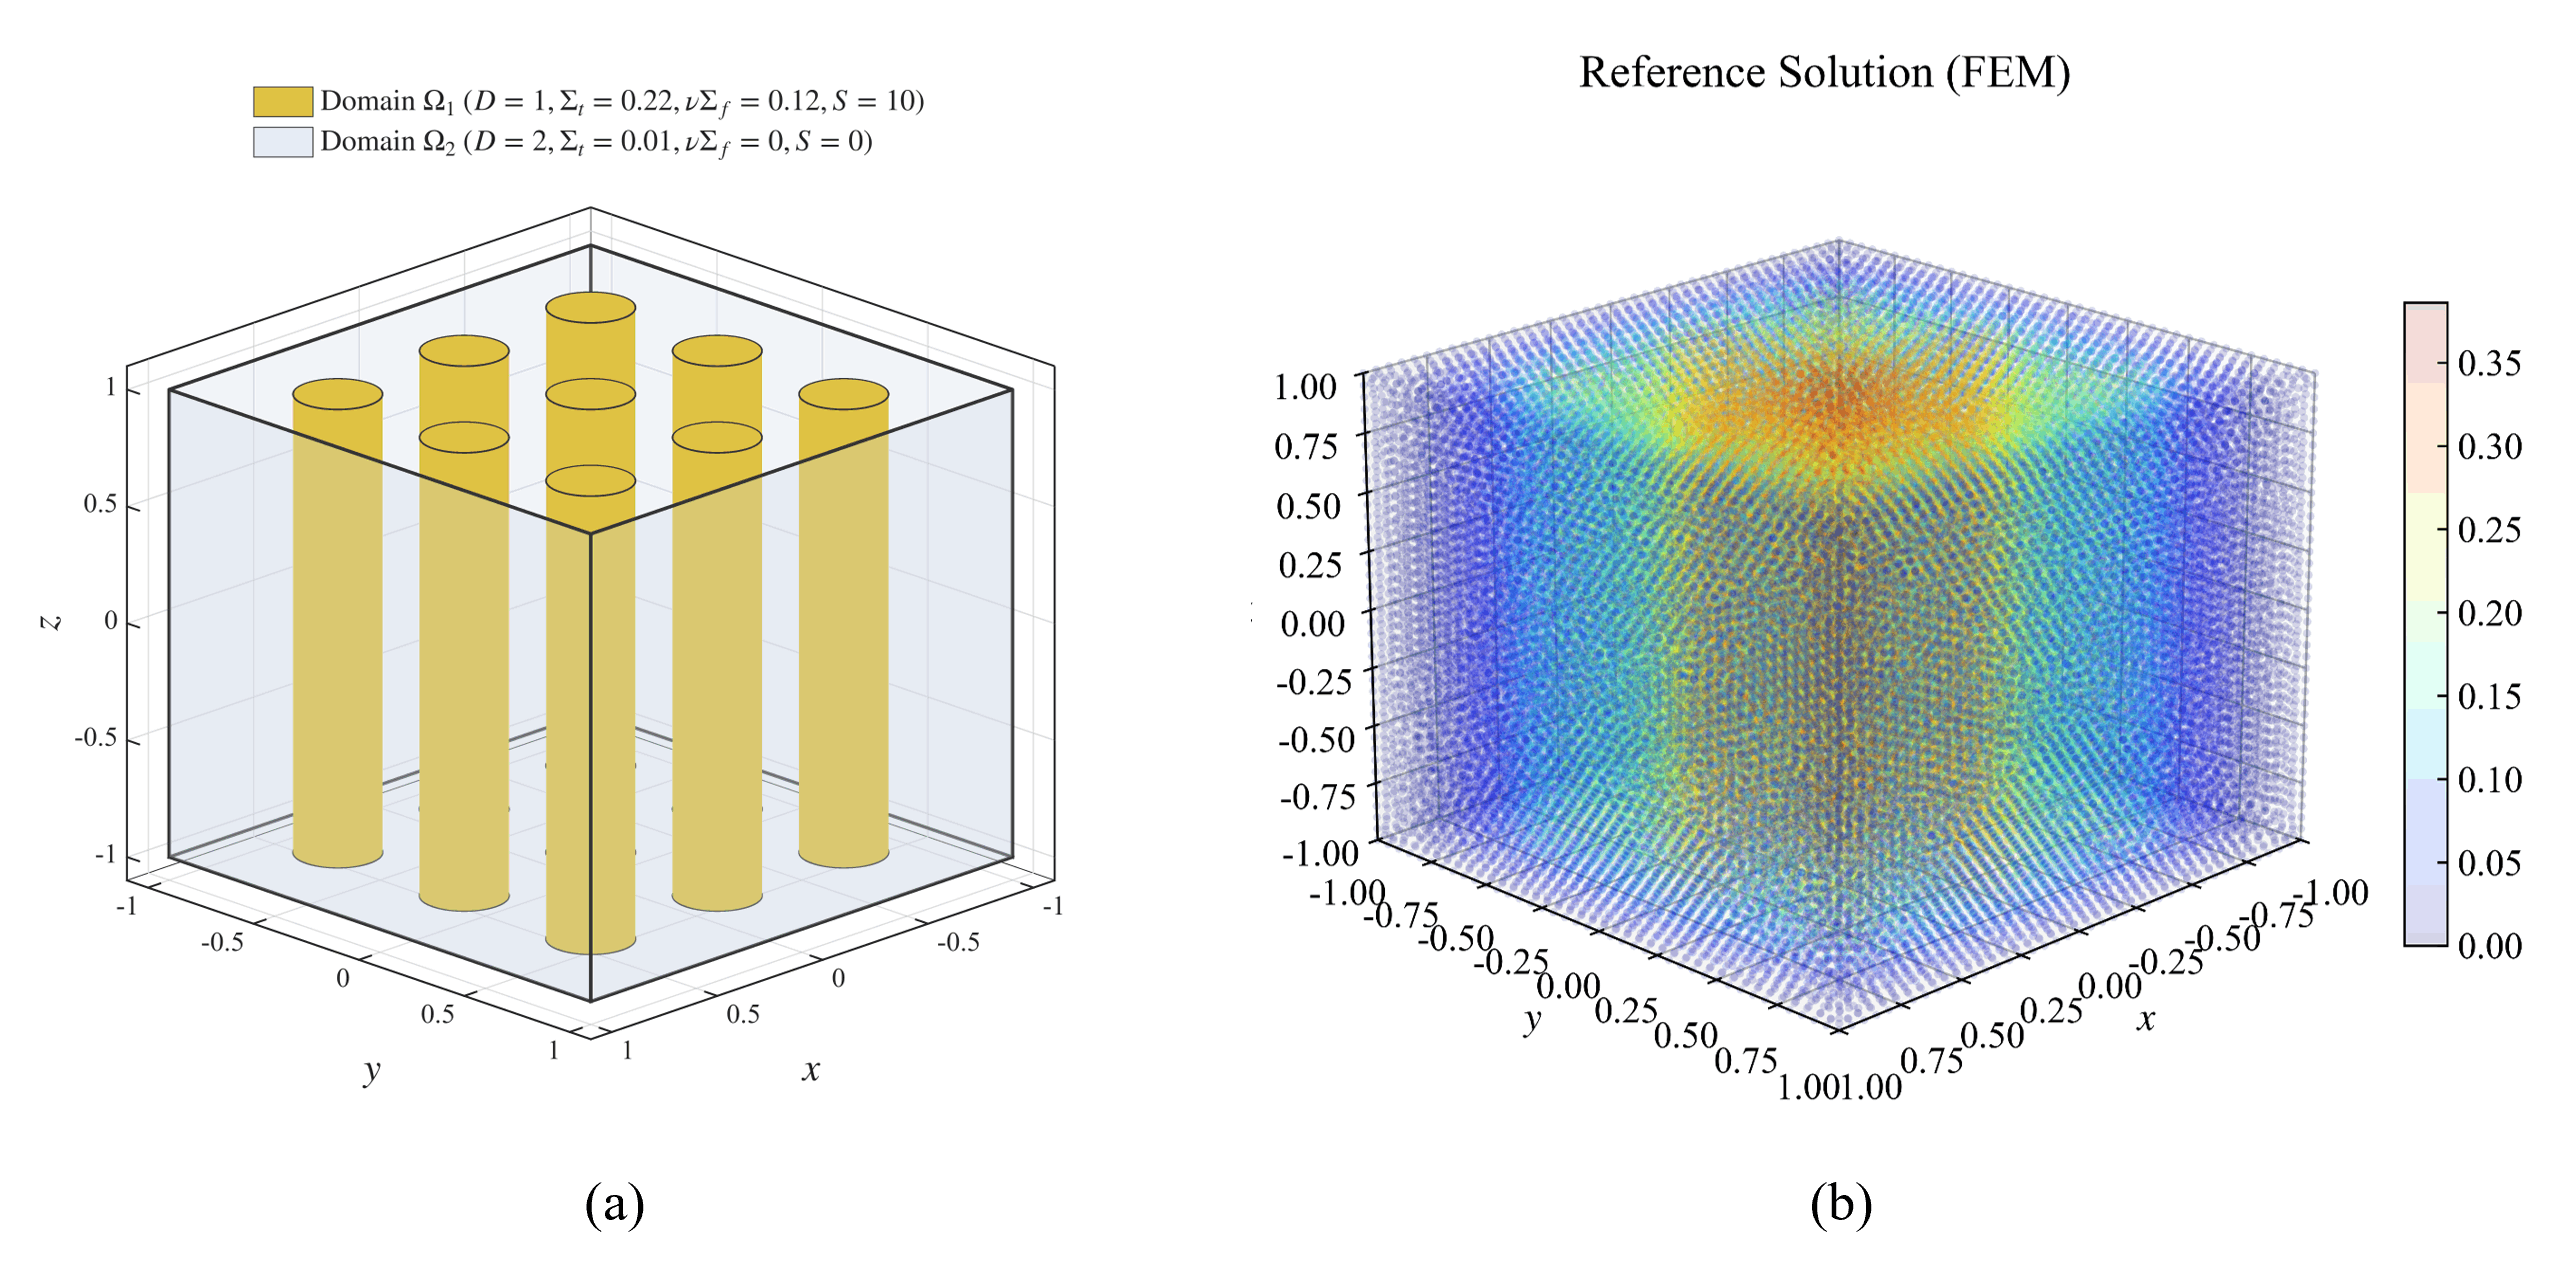
\includegraphics[width=0.7\textwidth]{fig/figure_07.png}
    \caption{算例 3：3D 圆柱棒束阵列单群固定源问题的计算设置。(a) 几何与材料分区；(b) FEM 参考通量。}
    \label{fig:case3_geometry_reference}
\end{figure}

本算例测试函数取 $v=1$，其余超参数与算例 2 保持一致。\cref{fig:case3_flux_error_comparison} 给出了标准 PINN 与 VIWS 的通量预测和误差分布。标准 PINN 的相对 $L_2$ 误差为 $3.55\times10^{-1}$，VIWS 的相对 $L_2$ 误差为 $6.26\times10^{-2}$。\cref{fig:case3_antiderivative_fields} 给出了对应原函数 $F_0$、$F_1$、$F_2$ 和 $F_3$。

\begin{figure}[H]
    \centering
    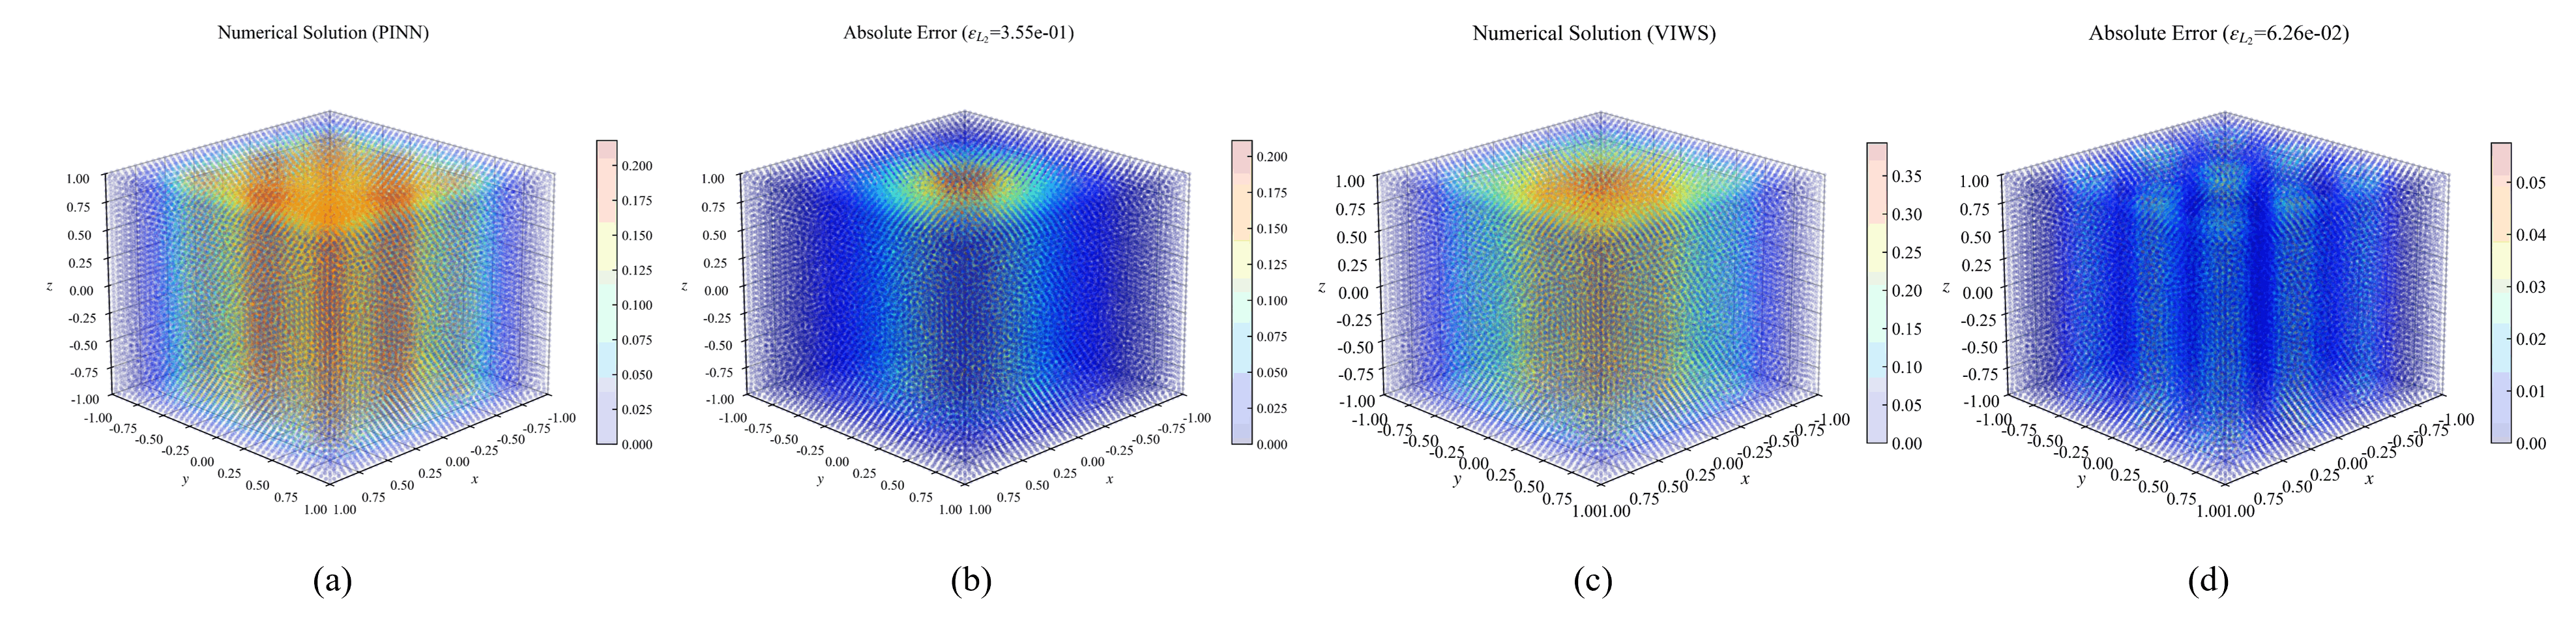
\includegraphics[width=1\textwidth]{fig/figure_08.png}
    \caption{算例 3：3D 圆柱棒束阵列单群固定源问题的通量预测与误差对比。(a) PINN 预测通量；(b) PINN 绝对误差；(c) VIWS 预测通量；(d) VIWS 绝对误差。}
    \label{fig:case3_flux_error_comparison}
\end{figure}

\begin{figure}[H]
    \centering
    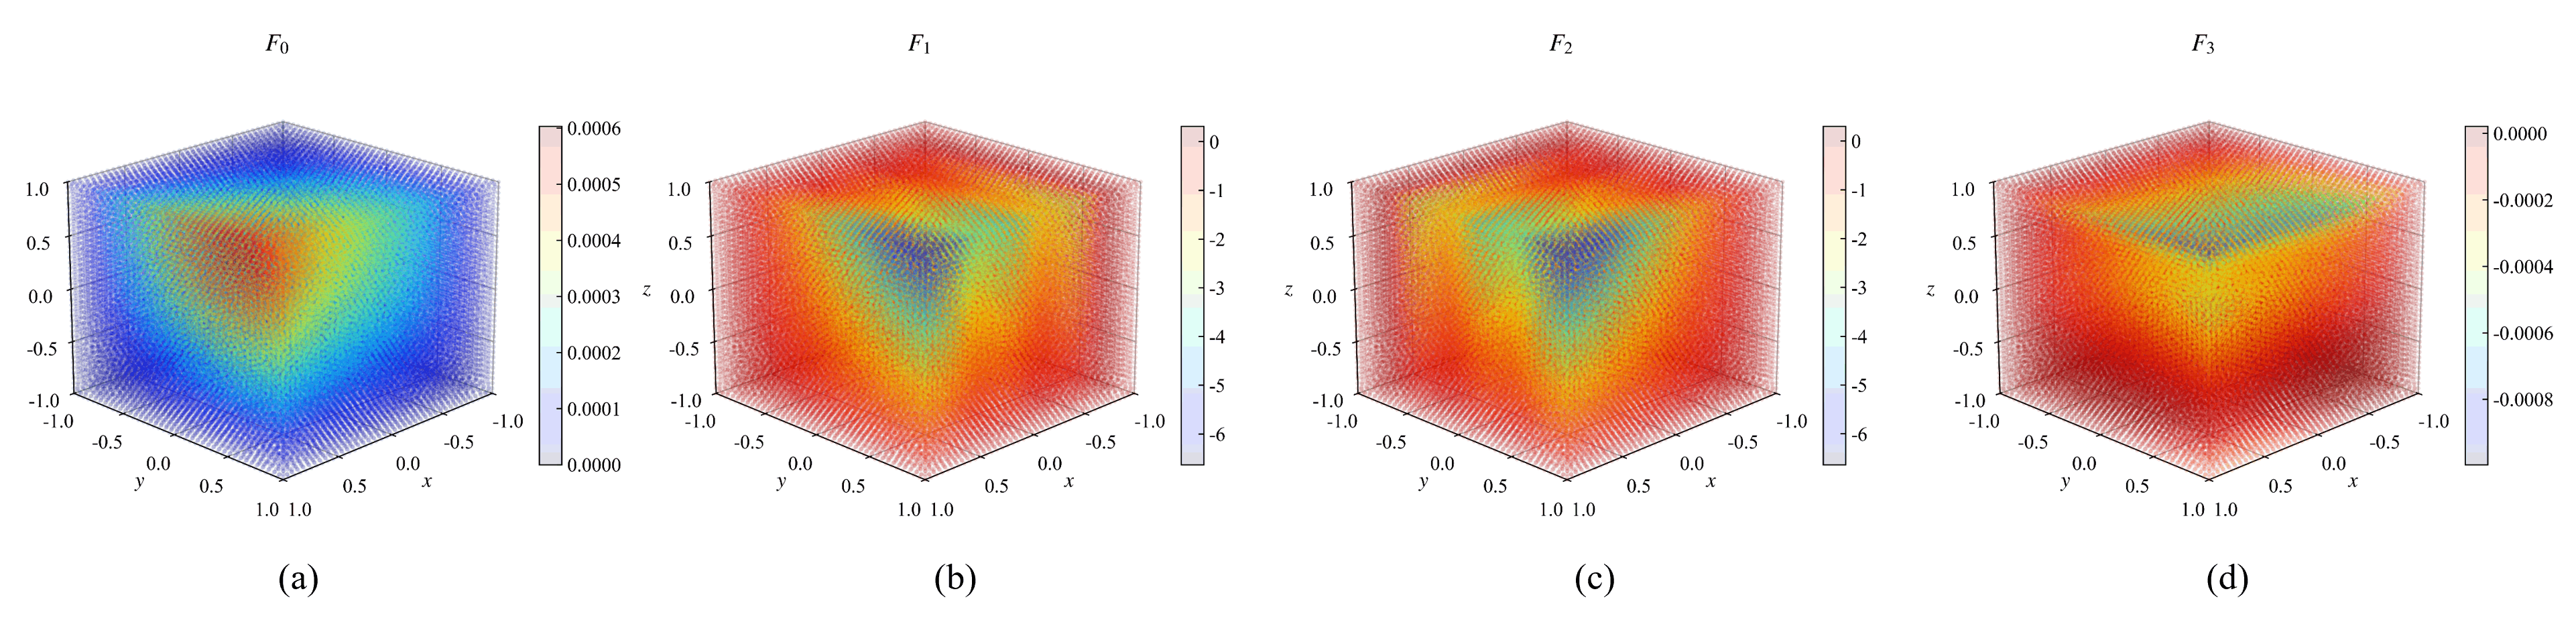
\includegraphics[width=1\textwidth]{fig/figure_09.png}
    \caption{算例 3：3D 圆柱棒束阵列单群固定源问题的原函数场。(a) $F_0$；(b) $F_1$；(c) $F_2$；(d) $F_3$。}
    \label{fig:case3_antiderivative_fields}
\end{figure}

结果表明，VIWS 可有效求解高维复杂几何界面问题，并能够处理 Dirichlet 与 Neumann 混合边界条件。

%=============================================================
\subsection{算例 4：2D L 形区域两群固定源问题}
\label{subsec:case4}

本算例进一步考察非规则几何中的两群耦合固定源问题。快群和热群通量分别记为 $\phi_1$ 和 $\phi_2$，空间坐标为 $\boldsymbol r=(x,y)$。控制方程为
\begin{equation}
    \begin{aligned}
        -\nabla \cdot \left( D_1 \nabla \phi_1(\boldsymbol r) \right)
        +\left(\Sigma_{\mathrm a,1} + \Sigma_{\mathrm s,1\rightarrow2}\right)\phi_1(\boldsymbol r)
         & =
        \nu_{1}\Sigma_{\mathrm f,1}\phi_1(\boldsymbol r)
        +\nu_{2}\Sigma_{\mathrm f,2}\phi_2(\boldsymbol r)
        +S_1(\boldsymbol r), \\
        -\nabla \cdot \left( D_2 \nabla \phi_2(\boldsymbol r) \right)
        +\Sigma_{\mathrm a,2}\phi_2(\boldsymbol r)
         & =
        \Sigma_{\mathrm s,1\rightarrow2}\phi_1(\boldsymbol r)
        +S_2(\boldsymbol r),
    \end{aligned}
    \label{eq:case4}
\end{equation}
其中 $D_g$ 为第 $g$ 群扩散系数，$\nu_g\Sigma_{\mathrm f,g}$ 为裂变产生截面，$S_g$ 为固定源项。

计算域为二维 L 形区域，由三个材料子区 $\Omega_1$、$\Omega_2$ 和 $\Omega_3$ 组成。\cref{fig:case4_geometry_reference}(a) 给出几何与材料分区，\cref{fig:case4_geometry_reference}(b) 和~\cref{fig:case4_geometry_reference}(c) 分别给出快群和热群 FEM 参考通量。两群材料参数列于~\cref{tab:case4_material_parameters}。

\begin{table}[H]
    \centering
    % \small
    \caption{算例 4：2D L 形区域两群固定源问题的材料参数}
    \label{tab:case4_material_parameters}
    \begin{tabularx}{0.95\textwidth}{@{\extracolsep{\fill}}ccccccc}
        \toprule
        子域
         & 能群
         & $D_g$ (cm)
         & $\Sigma_{\mathrm a,g}$ (cm$^{-1}$)
         & $\nu_g\Sigma_{\mathrm f,g}$ (cm$^{-1}$)
         & $\Sigma_{\mathrm s,1\rightarrow2}$ (cm$^{-1}$)
         & $S_g$                                                                                      \\
        \midrule
        $\Omega_1$
         & 1                                              & 1.255  & 0.013052 & 0.00480 & 0.02533 & 1 \\
         & 2                                              & 0.2110 & 0.10030  & 0.00000 &         & 0 \\

        $\Omega_2$
         & 1                                              & 1.268  & 0.011501 & 0.00432 & 0.02767 & 0 \\
         & 2                                              & 0.1902 & 0.07047  & 0.00000 &         & 0 \\

        $\Omega_3$
         & 1                                              & 1.259  & 0.012562 & 0.00456 & 0.02617 & 0 \\
         & 2                                              & 0.2091 & 0.08344  & 0.00000 &         & 0 \\
        \bottomrule 
    \end{tabularx}
\end{table}

\begin{figure}[H]
    \centering
    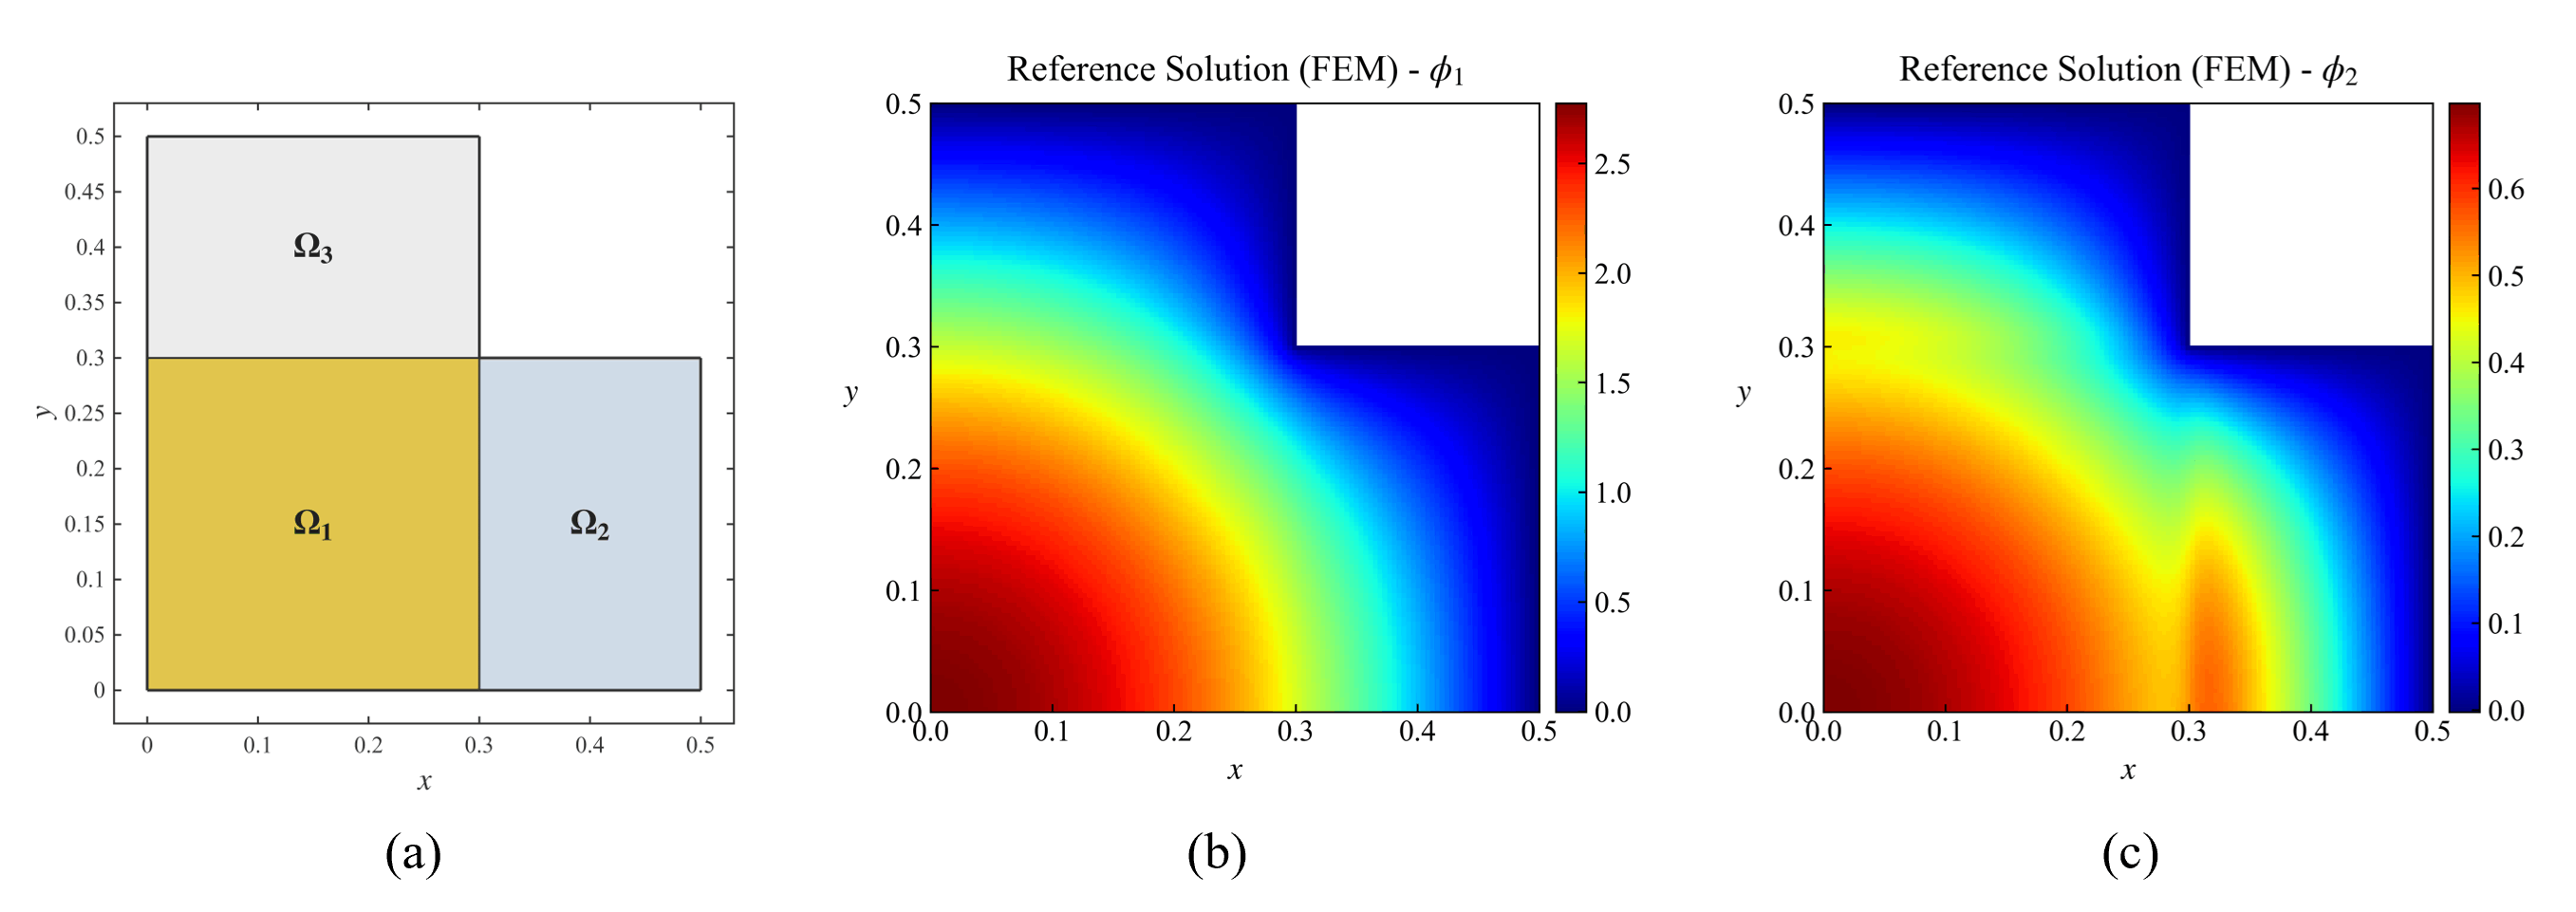
\includegraphics[width=0.8\textwidth]{fig/figure_10.png}
    \caption{算例 4：2D L 形区域两群固定源问题的计算设置。(a) 几何与材料分区；(b) 快群 FEM 参考通量；(c) 热群 FEM 参考通量。}
    \label{fig:case4_geometry_reference}
\end{figure}

右边界和上边界施加零通量 Dirichlet 条件，左边界和下边界施加零法向流 Neumann 条件：
\begin{equation}
    \begin{aligned}
        \phi_g(\boldsymbol r)                         & = 0,
                                                      &      & \boldsymbol r\in\partial\Omega_{\mathrm D}, \\
        \nabla\phi_g(\boldsymbol r)\cdot\boldsymbol n & = 0,
                                                      &      & \boldsymbol r\in\partial\Omega_{\mathrm N},
    \end{aligned}
    \qquad g=1,2 ,
    \label{eq:case4_bc}
\end{equation}
其中 $\boldsymbol n$ 为单位外法向量，$\partial\Omega_{\mathrm D}$ 和 $\partial\Omega_{\mathrm N}$ 分别表示 Dirichlet 边界和 Neumann 边界。

本算例采用两个独立神经网络分别表示 $\phi_1$ 和 $\phi_2$，测试函数取 $v=x+y+1$，域内均匀采样 $13,783$ 个点。\cref{fig:case4_flux_error_comparison} 给出 VIWS 对快群和热群通量的预测结果及绝对误差。快群和热群相对 $L_2$ 误差分别为
$\epsilon_{L_2}^{(1)}=4.66\times10^{-3}$ 和
$\epsilon_{L_2}^{(2)}=2.10\times10^{-2}$，较大误差主要位于 L 形凹角附近。结果说明，VIWS 能够处理非规则几何中的两群耦合固定源问题。

\begin{figure}[H]
    \centering
    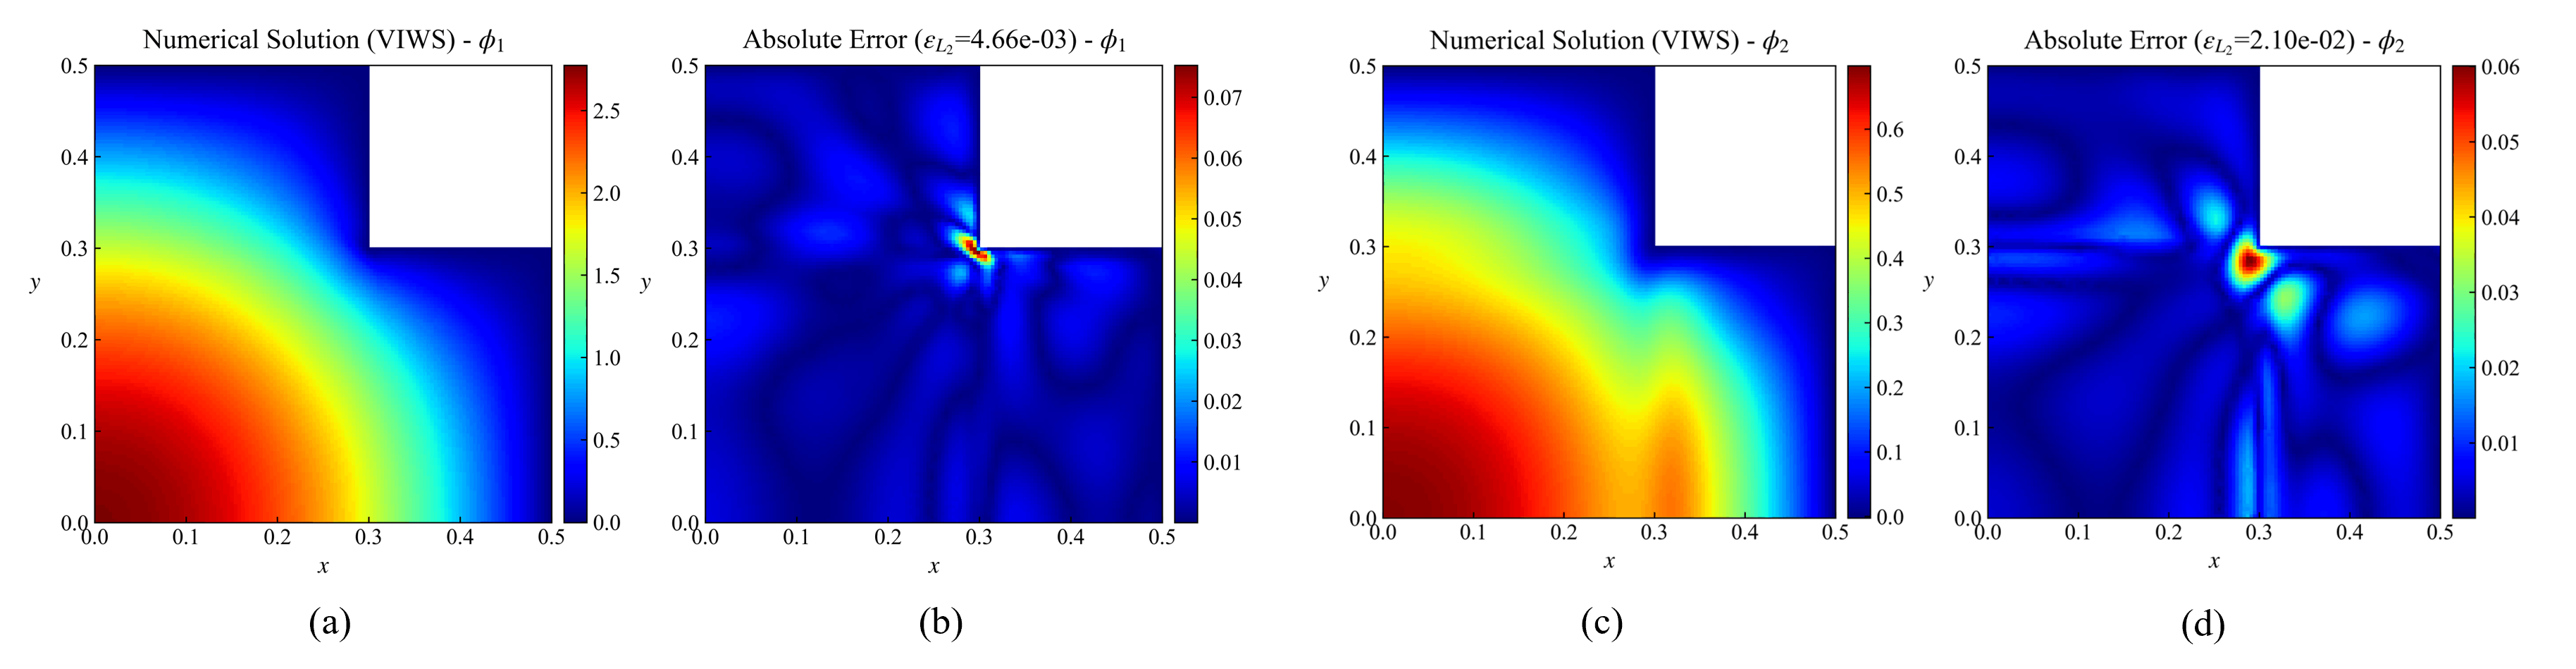
\includegraphics[width=1\textwidth]{fig/figure_11.png}
    \caption{算例 4：2D L 形区域两群固定源问题的 VIWS 通量预测与误差分布。(a) 快群预测通量；(b) 快群绝对误差；(c) 热群预测通量；(d) 热群绝对误差。}
    \label{fig:case4_flux_error_comparison}
\end{figure}

%=============================================================
\subsection{算例 5：2D-IAEA 两群中子扩散特征值基准题}
\label{subsec:case5}
本算例选取经典的 2D-IAEA 压水堆（PWR）两群中子扩散特征值基准题，旨在验证 VIWS 框架在处理复杂多材料几何及特征值问题的适用性。该问题忽略了缓发中子先驱核的影响~\cite{theler2011solution}，其控制方程及对应的变域积分弱形式分别见~\cref{eq:two_group_eigenvalue} 与~\cref{eq:two_group_variable_weak_form}。在堆芯配置方面，该基准题由两类燃料区与外部反射层组成，共计 177 个燃料组件；单个组件宽度为 $20\,\mathrm{cm}$，外围反射层厚度亦为 $20\,\mathrm{cm}$。基于几何结构与材料分布的对称性，计算中仅取其四分之一区域，该区域涵盖 $\Omega_1$--$\Omega_4$ 四类材料子区，具体排布如图~\cref{fig:case5_geometry_reference}(a) 所示。边界条件设定如下：对称边界采用零法向流 Neumann 条件，外部边界则采用零通量 Dirichlet 条件。相关材料群常数详见~\cref{tab:case5_material_parameters}。此外，图~\cref{fig:case5_geometry_reference}(b) 与 (c) 分别给出了基于有限元法（FEM）获得的快群与热群参考通量分布，对应的参考有效增殖因子为 $k_{\mathrm{eff}}=1.03394$。

\begin{table}[H]
    \centering
    % \small
    \caption{算例 5：2D-IAEA 两群中子扩散特征值基准题的材料参数}
    \label{tab:case5_material_parameters}
    \begin{tabularx}{0.95\textwidth}{@{\extracolsep{\fill}}ccccccc}
        \toprule
        子域
         & 能群
         & $D_g$ (cm)
         & $\Sigma_{\mathrm a,g}$ (cm$^{-1}$)
         & $\nu_g \Sigma_{\mathrm f,g}$ (cm$^{-1}$)
         & $\Sigma_{\mathrm s,1\rightarrow2}$ (cm$^{-1}$)
         & 材料                                                                                       \\
        \midrule
        $\Omega_1$
         & 1                                              & 1.5 & 0.010 & 0.000 & 0.02 & 燃料 1       \\
         & 2                                              & 0.4 & 0.080 & 0.135 &      &            \\
        $\Omega_2$
         & 1                                              & 1.5 & 0.010 & 0.000 & 0.02 & 燃料 2       \\
         & 2                                              & 0.4 & 0.085 & 0.135 &      &            \\
        $\Omega_3$
         & 1                                              & 1.5 & 0.010 & 0.000 & 0.02 & 燃料 2 + 控制棒 \\
         & 2                                              & 0.4 & 0.130 & 0.135 &      &            \\
        $\Omega_4$
         & 1                                              & 2.0 & 0.000 & 0.000 & 0.04 & 反射层        \\
         & 2                                              & 0.3 & 0.010 & 0.000 &      &            \\
        \bottomrule 
    \end{tabularx}
\end{table}

\begin{figure}[H]
    \centering
    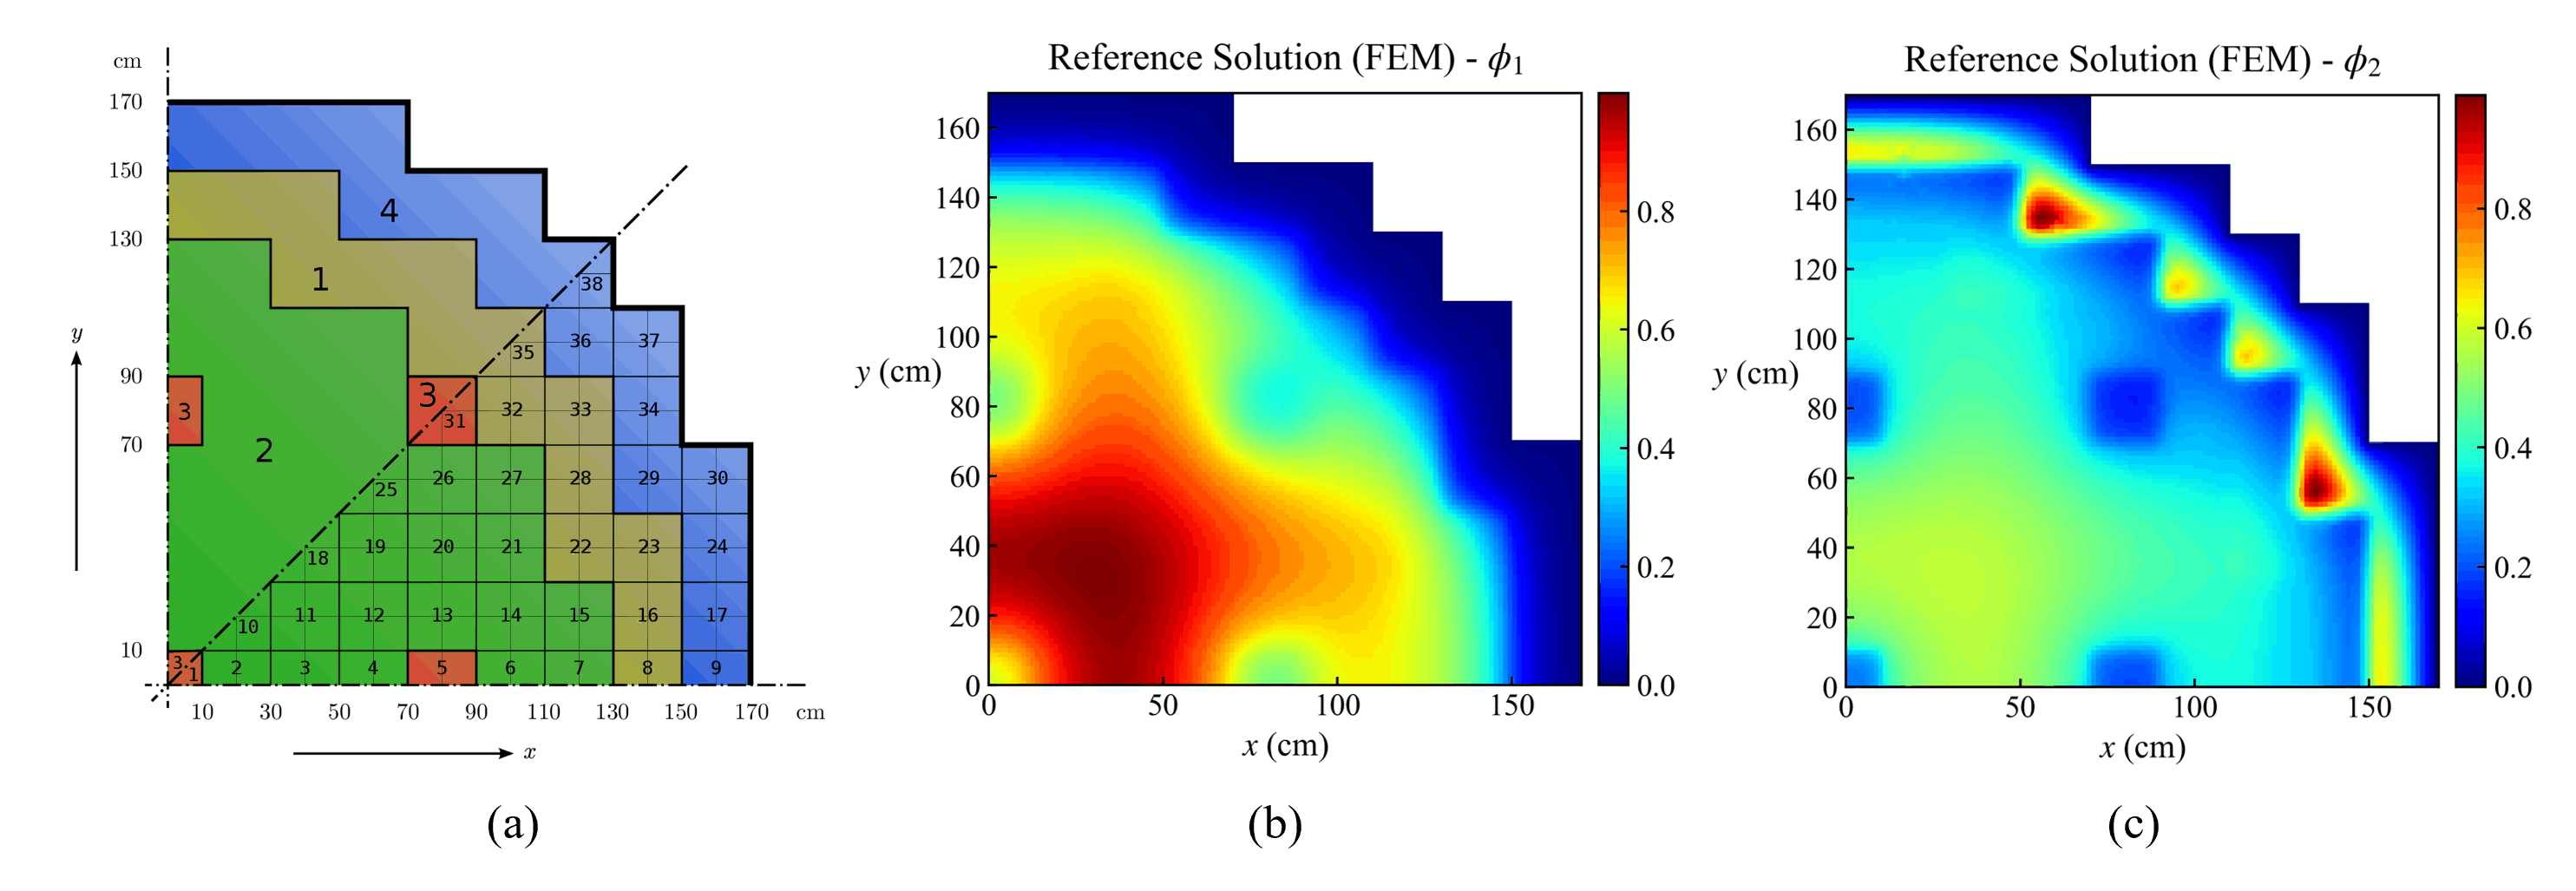
\includegraphics[width=0.8\textwidth]{fig/figure_12.png}
    \caption{算例 5：2D-IAEA 两群中子扩散特征值基准题的计算设置。(a) 四分之一堆芯几何与材料分区；(b) 快群 FEM 参考通量；(c) 热群 FEM 参考通量。}
    \label{fig:case5_geometry_reference}
\end{figure}

特征值问题的通量幅值具有尺度不唯一性\cite{LiuDong2022JiYupinnShen,LiuDong2023HeFanYing}。为固定特征函数幅值并避免平凡解，本文对快群通量施加全局归一化约束：
\begin{equation}
    \mathcal{L}_{\mathrm{norm}}
    =
    \left(
    \frac{1}{N_r}
    \sum_{i=1}^{N_r}
    \phi_1^2(\boldsymbol r_i)
    -1
    \right)^2 .
    \label{eq:loss_norm}
\end{equation}
同时，在网络输入端引入 Fourier 特征映射~\cite{tancik2020fourier}，以增强网络对材料界面、几何角点和局部高梯度区域的表征能力。有效增殖因子 $k_{\mathrm{eff}}$ 作为全局待优化参数，与神经网络权重同步更新。域内均匀采样 $54,677$ 个点，测试函数取 $v=1$。

~\cref{fig:case5_flux_error_keff} 给出了 VIWS 的两群通量预测、误差分布及 $k_{\mathrm{eff}}$ 收敛过程。计算得到
$k_{\mathrm{eff}}=1.03372$，与 FEM 参考值的偏差约为 $22\,\mathrm{pcm}$。快群和热群通量相对 $L_2$ 误差分别为
$\epsilon_{L_2}^{(1)}=4.01\times10^{-2}$ 和
$\epsilon_{L_2}^{(2)}=8.89\times10^{-2}$。结果说明，VIWS 能够用于具有工程几何特征的两群中子扩散特征值问题，并可同时给出有效增殖因子和对应通量场。

\begin{figure}[H]
    \centering
    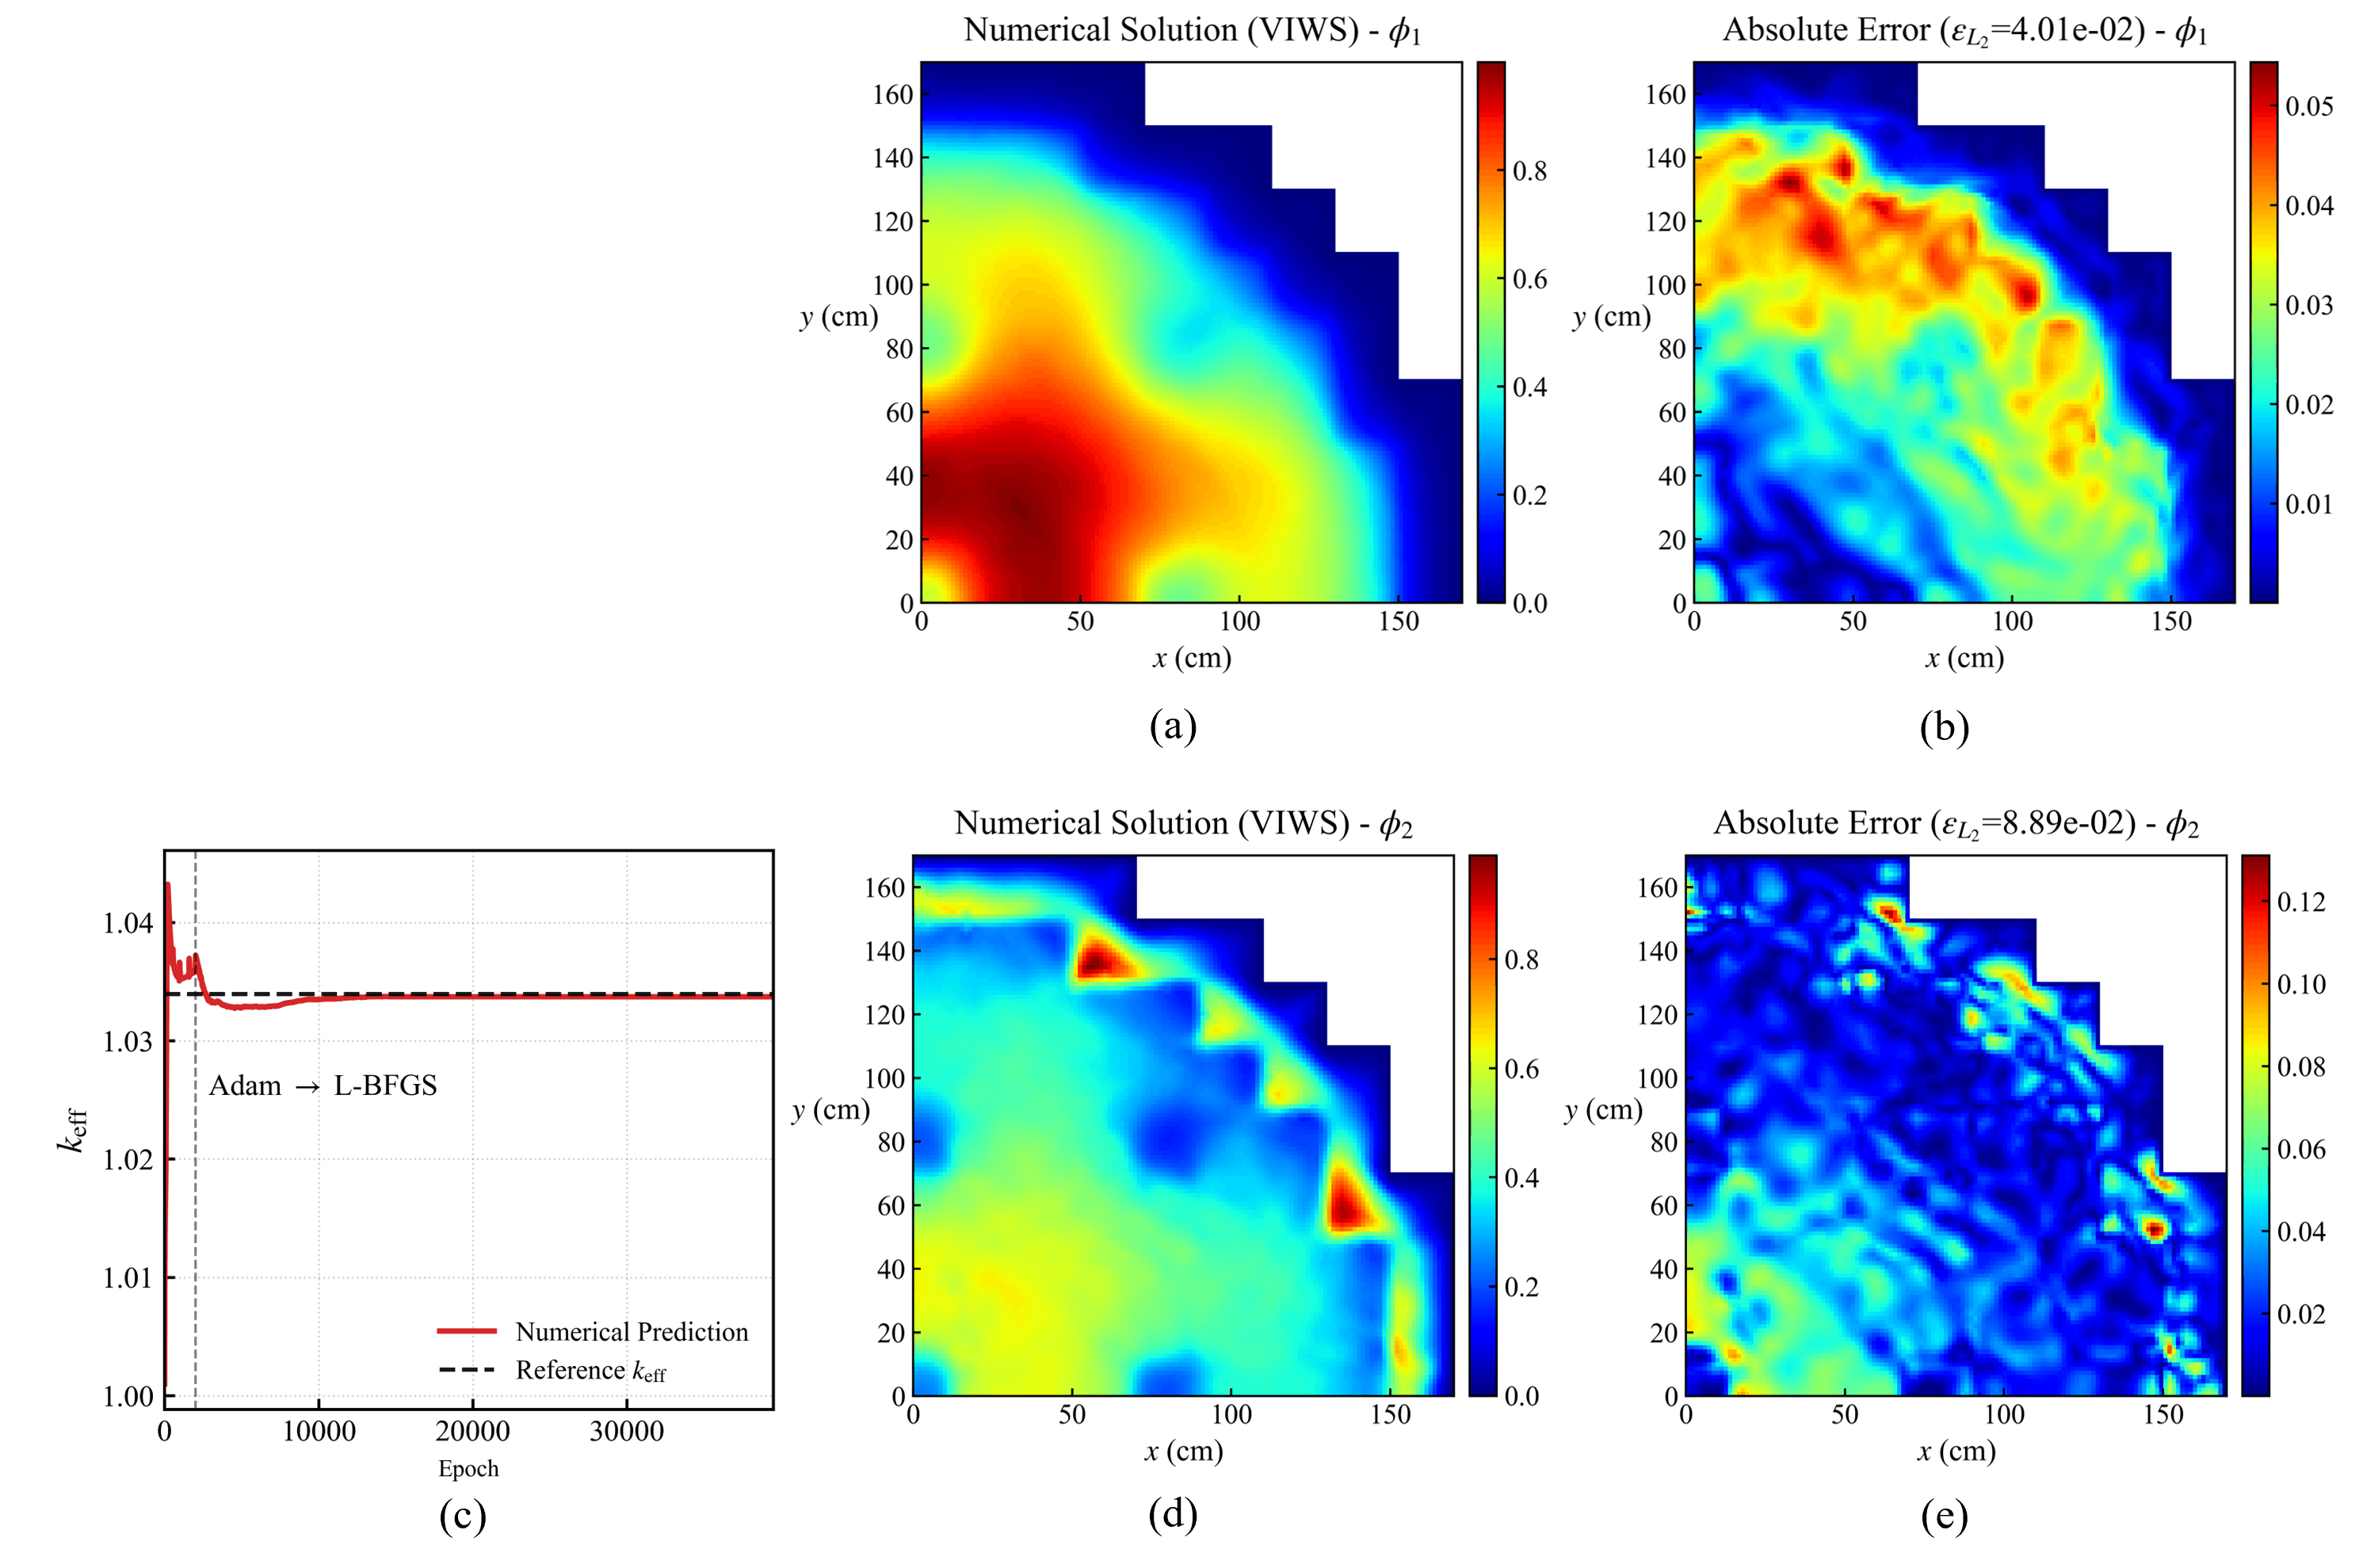
\includegraphics[width=0.8\textwidth]{fig/figure_13.png}
    \caption{算例 5：2D-IAEA 两群中子扩散特征值基准题的 VIWS 计算结果。(a) 快群预测通量；(b) 快群绝对误差；(c) $k_{\mathrm{eff}}$ 收敛曲线；(d) 热群预测通量；(e) 热群绝对误差。}
    \label{fig:case5_flux_error_keff}
\end{figure}


\section{结论}
\label{sec:conclusion}
本文针对非均匀介质中子扩散计算中材料系数不连续引起的界面梯度跳变问题，将变域积分弱解（VIWS）理论应用于中子扩散方程的深度学习求解。本文主要贡献如下：
首先，通过在分部积分过程中引入变域积分区域，构造了适用于复杂几何和多群条件的中子扩散方程变域积分弱形式，从而有效缓解中子扩散方程求解中界面导数奇异性带来的困难，并提高计算精度。其次，采用单一神经网络表示中子扩散方程全局数值解，基于通量连续原理，隐式处理了界面导数跳变问题，避免了复杂内部界面条件的显式处理。最后，针对具有连续核函数的积分项，进一步将其转化为相应的原函数形式并用于深度学习求解，从而提升了计算效率。

数值结果表明，本文所提方法在处理二维和三维非均匀介质中子扩散问题时具有良好的精度，显著优于经典PINN方法。适用于非规则边界、混合边界条件、多群耦合以及特征值计算，具有良好的工程应用潜力。

未来研究可重点关注将本文所提方法扩展到三维时空中子动力学问题、多物理场耦合和大规模反应堆复杂堆芯问题等实际应用中。此外，未来还可结合新一代神经网络架构以及大规模并行计算的机器学习等方法，以持续提升深度学习方法在中子扩散计算中的精度和效率，推进实际工程应用。


\section*{Acknowledgments}
This research is supported by the National Natural Science Foundation of China (Grant No. 12575189), the Basic Research and Stable Support Research Project of Science and Technology Industry Bureau of China (Grant No. WDZC2023050305) and the Supported by Sichuan Science and Technology Program (Grant No. 2023YFG0373).

% \newpage
\bibliographystyle{elsarticle-num}
\bibliography{C:/Users/mathliuyang/Zotero/ref_BibTeX}

\end{document}

\endinput
%%
%% End of file `main.tex'.
